\chapter{项目实现}
\label{cha:project_implement}
本章详细介绍项目系统的实现,集中于介绍项目的三个创新点:子网信道隔离的部署方案、
跨层视频帧权重差分技术、路径质量敏感的动态切换阈值算法。
其中,子网信道隔离从整体网络规划上指导大型Mesh网络的架构;
跨层视频帧权重差分技术在将802.11系列标准的QoS技术引入,针对视频传输提供了强大的
QoS保障;路径质量敏感的动态切换阈值算法专注于优化Mesh节点移动带来的路径切换时延,并
有效抑制路由震荡现象。

本章工作基于细致全面的实验和对BATMAN-adv代码的在实际系统的定制开发和调试,最终带来网络
性能上的提升巨大。在系统实践中也积累了大量的无线网络规划经验和linux内核模块
开发调试的技术,为我们的多个对外项目的实施提供了指导。

\section{子网信道隔离}
\label{sec:1}
出于成本考虑,项目所选择的硬件平台仅支持单一无线接口,这就意味着每一个节点设备
同一时间只能工作在一个无线信道。而无线信道的开放性所带来的信道竞争排斥多路并发传输。
不同的无线终端在进行数据传输之前需要先竞争使用信道。这个阶段称为信道接入。

在802.11定义了基本的信道接入方式:分布式协调功能,该方式本质上就是一种CSMA/CA
机制。CSMA机制在工业界广泛使用,比如以太网中使用的CSMA/CD,
其中CD表示冲突检测。在无线网络中,因为隐终端的存在,CD的方式不可靠,因此多使用CA的
方式。CSMA/CA工作流程
如下:当一个终端需要占用信道发送数据时,如果信道繁忙(其他终端正在使用信道),那么就会
推迟一段时间进行下一次尝试,如果信道检测为空闲就可以立即发送数据。

\subsection{相邻链路干扰}
因为信道竞争和隐终端的影响,如果所有节点选择同一信道则会造成严重的信道干扰,导致网络总体
吞吐量的急剧下降。
\begin{figure}[H] % use float package if you want it here
  \centering
  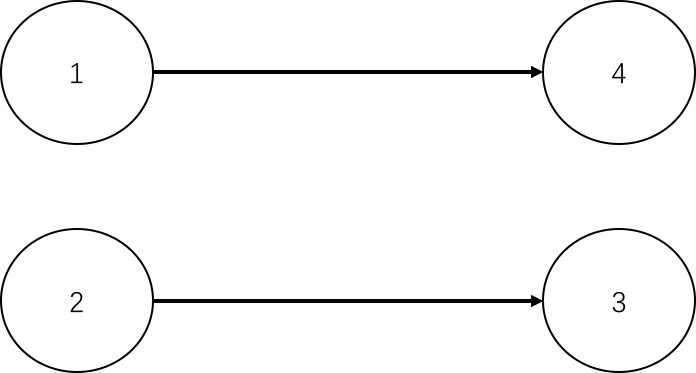
\includegraphics[width=0.4\textwidth]{interference}
  \caption{相邻链路干扰实验图示}
  \label{fig:interference}
\end{figure}

首先是相邻链路的信道竞争。图~\ref{fig:interference}给出了实验图示,节点1和节点4之间通信的同时
节点2和节点3通信,产生信道竞争,导致每条链路的实际有效带宽下降。
实验结果如下表~\ref{tab:interference}所示。

\begin{table}[htbp]
  \centering
  \caption{相邻链路干扰实验结果}
  \label{tab:interference}
  \begin{tabular}{p{2cm}p{2cm}p{2cm}p{2cm}p{2cm}p{2cm}}
  \hline
  发送功率 & 信道(L1-L2) & L1单独实际带宽(Mbps) & L2单独实际带宽(Mbps) & L1并发实际带宽(Mbps) & L2并发实际带宽(Mbps) \\
  \hline
  27 &  149-153 & 54.2 & 54 & 29.1 & 27.2 \\
  8 &  149-153 & 54.1 & 54.2 & 27.8 & 29.1 \\
  6 &  149-153 & 52.5 & 54.7 & 27.5 & 30 \\
  5 &  149-153 & 54.3 & 54.2 & 29.4 & 28.4 \\
  2 &  149-153 & 43.9 & 46.1 & 30.5 & 32.1 \\
  \hline
  \end{tabular}
\end{table}

可以明显看出当两条相邻链路同时发送数据时,各自的吞吐量降为原先的一半左右,当相邻的并发链路数量过多时
即可能导致每条链路的实际吞吐不足以支持视频流传输。

\subsection{隐终端}
隐终端指当网络中存在多个终端时,某终端只能在信道竞争时获知相邻终端的存在,而无法感知其他
更远处终端的存在,处于远处的未被感知的终端即称为隐终端。当某终端侦听信道判断当前信道空闲时,就会发送
数据,但可能与此同时远处的隐终端也认为信道空闲并发送数据,假设此时两份数据的接收者处于两者的物理位置
的中间,则两份数据同时到达将造成混乱,无法分辨,从而无法应答。导致两边的终端不得不反复的重传,甚至发生
数据包丢失。以下实验就是探究隐终端在Mesh网络中的影响。

首先进行单跳实验,网络拓扑如图~\ref{fig:hiddenterminal-1}。客户端连接1节点,服务端连接
5节点,图中共计5个节点组成一个稳定的无线Mesh网络。

在客户端和服务端之间,通过Mesh网络进行100次测试。每次测试运行20秒,客户端上的发送进程分别
以1至100间隔1Mbps的发送带宽向服务端发送UDP数据包。每次测量结束,服务端上的服务进程会统计
客户端此次通信数据的有效带宽、时延抖动等数据并告知客户端进程。所有测量结果在客户端汇总整理。

然后进行隐终端存在的实验,网络拓扑如图~\ref{fig:hiddenterminal-2}。客户端机器通过交换机与
Mesh网络中的1节点和5节点连接,服务端机器与Mesh网络中的3节点相连,在该网络中,1节点和
5节点互相不在覆盖范围内,不知道对方的存在。
在客户端和服务端之间,客户端
虚拟两个进程,利用Iperf工具并控制1节点和5节点并发向3节点发送数据,调节发射功率从500次
依次增大到1700,每次通过Mesh网络进行100次测试。每次测试进行20秒,客户端上的两个进程分别以
1到100间隔1Mbps的发送带宽向服务端发送UDP数据包。每次测量结束,服务端的进程统计客户端进程
此次通信数据的有效带宽等数据并告知客户端进程。所有测量结果在客户端汇总整理。
以上实验过程在1节点和5节点RTS/CTS打开与关闭的情况下分别进行一次。

\begin{figure}[H] % use float package if you want it here
  \centering
  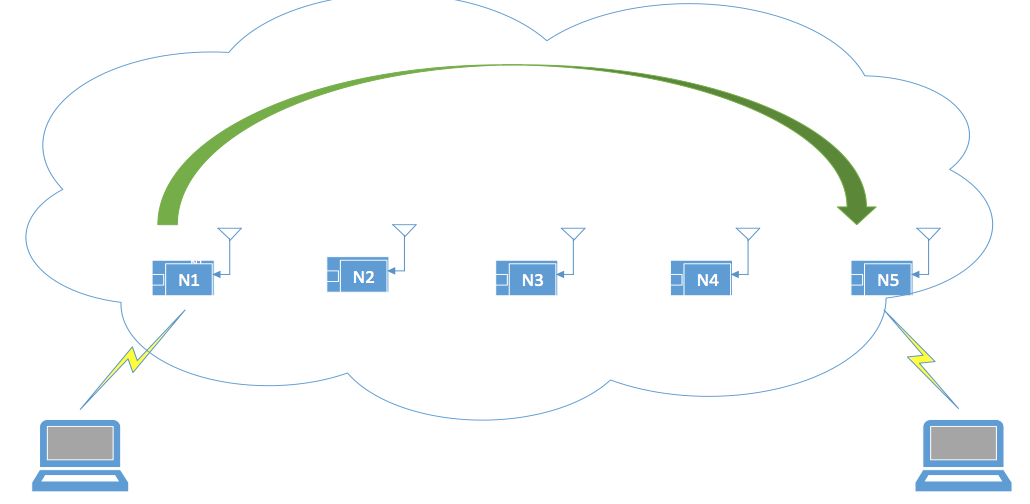
\includegraphics[width=0.6\textwidth]{hiddenterminal-onehop}
  \caption{单跳带宽测试}
  \label{fig:hiddenterminal-1}
\end{figure}
\begin{figure}[H] % use float package if you want it here
  \centering
  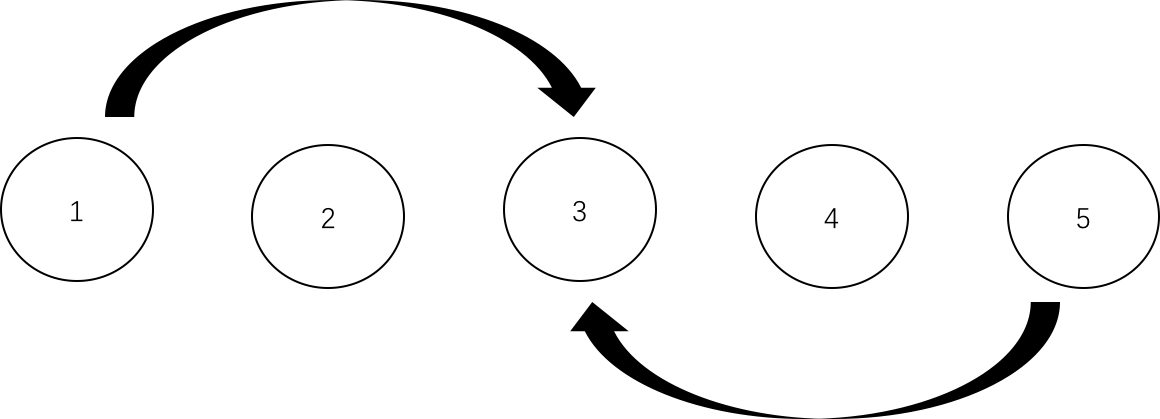
\includegraphics[width=0.6\textwidth]{hiddenterminal-hidden}
  \caption{隐终端带宽测试}
  \label{fig:hiddenterminal-2}
\end{figure}

单跳带宽测试实验结果如图~\ref{fig:hiddenterminal-3}所示,可以看到
在无干扰情况下,硬件平台支持的最大带宽约95Mbps。

相较之下,隐终端存在的带宽测试实验结果如图~\ref{fig:hiddenterminal-4}所示,
该图示中同时呈现了RTS/CTS打开和关闭情况下实际有效带宽。可以明显看出RTS/CTS打开情况,实际有效
带宽提升在10Mbps至20Mbps。但考虑到RTS/CTS打开,因为需要发送RTS/CTS控制帧,所以会造成一定
程度上的额外资源开销。

进一步引入发送功率
作为因变量。之所以考虑发送功率,是因为发送功率和干扰范围密切相关,当发送功率升高时,
其干扰范围就会扩大,很大可能导致网络整体吞吐量下降。反之,发送功率过小,则会导致网络形成
更多的多跳路由,而每多一跳同样会带来额外的干扰。我们对发送功率同样进行了实验
辅助建模,探索其和有效带宽的关系。

实验结果如图图~\ref{fig:hiddenterminal-5}所示,可以发现当发送带宽较小,即使较小的发送功率
也可以满足要求。但当发送带宽超过50Mbps后,发送功率就会成为限制有效带宽的一个重要因素,随着
发送功率进一步增大,有效带宽逐渐达到饱和。因此,在实际部署时,需要权衡所需的单节点
最高需求带宽和可承受的最大干扰范围。如果需要的单节点最大带宽在50Mbps之内,发送功率
就可以控制在8左右,如果大雨50Mbps,发送功率需要达到10。

综合发送带宽和发送功率绘制图~\ref{fig:hiddenterminal-6}。可以看到RTS/CTS打开的情况下,
有效带宽呈现出更好的状态。因此在实际项目系统的测试和部署中,如不特殊说明,将选择打开RTS/CTS
功能。

\begin{figure}[h]
  \centering
  \subcaptionbox{单跳带宽测试实验结果\label{fig:hiddenterminal-3}}
      {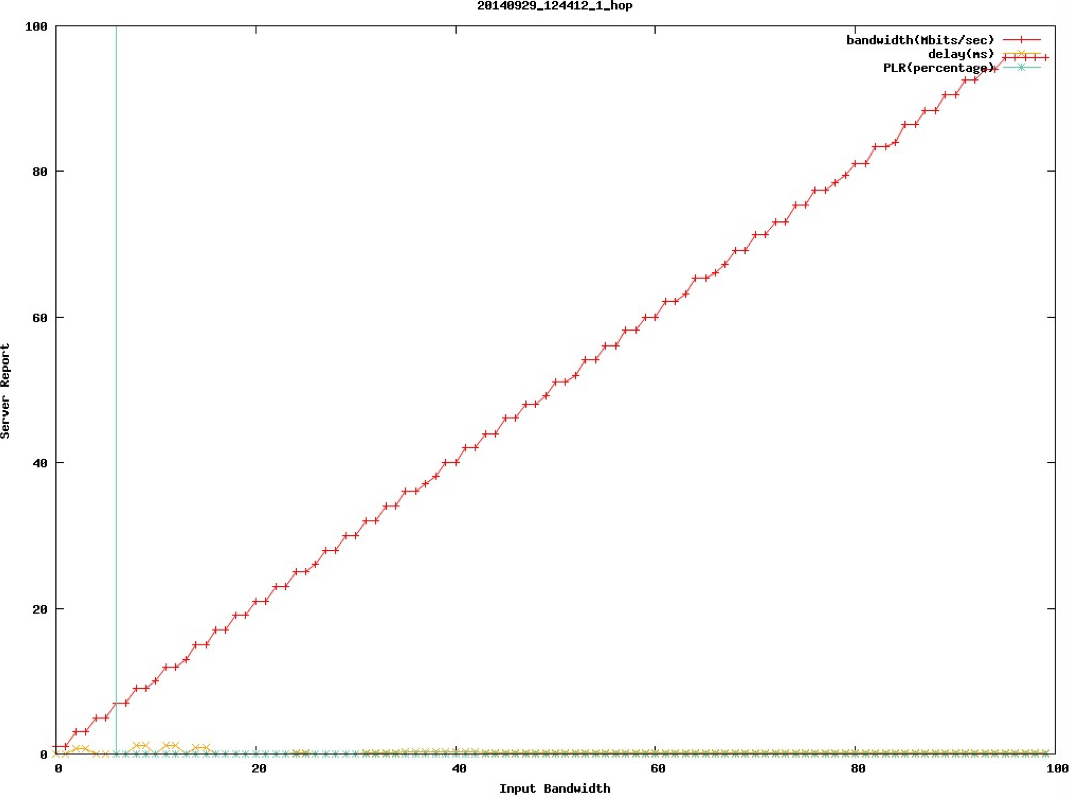
\includegraphics[height=5cm]{hiddenterminal-onehop-result}}
  \hspace{1em}
  \subcaptionbox{隐藏终端带宽测试实验结果(rts打开vsrts关闭)\label{fig:hiddenterminal-4}}
    {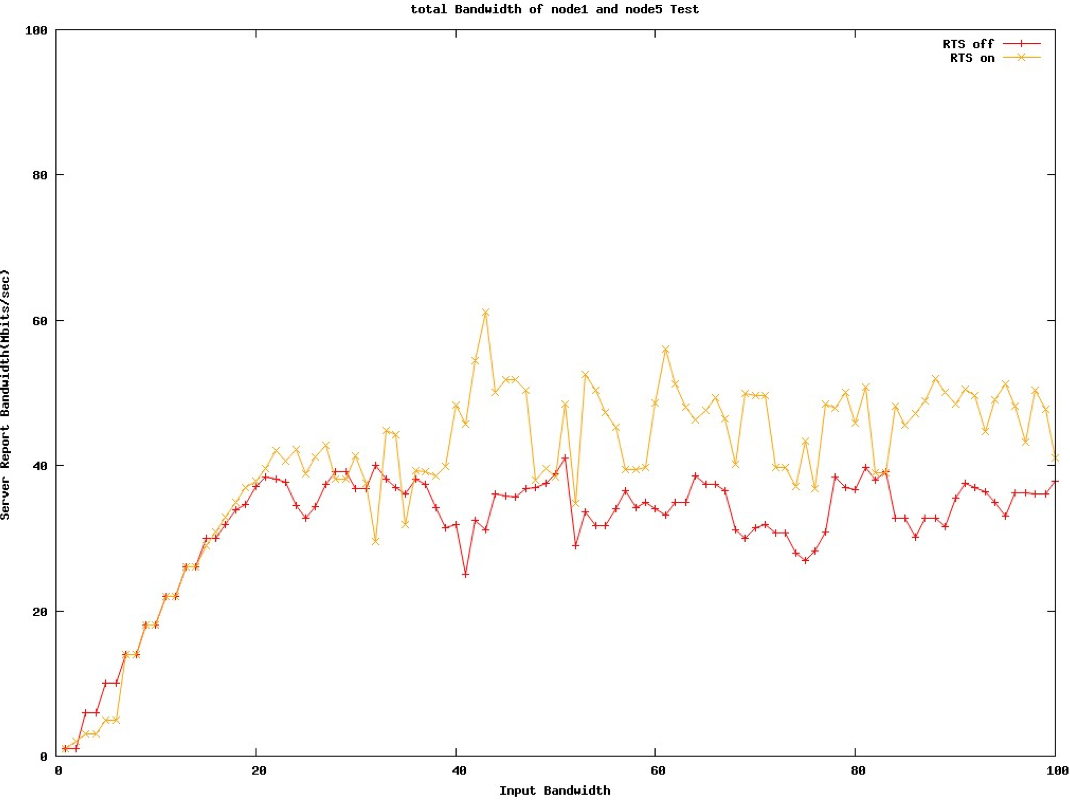
\includegraphics[height=5cm]{hiddenterminal-rts-comp}}
  \caption{带宽测试结果}
\end{figure}

\begin{figure}[h]
  \centering
  \subcaptionbox{发送功率对带宽的影响\label{fig:hiddenterminal-5}}
      {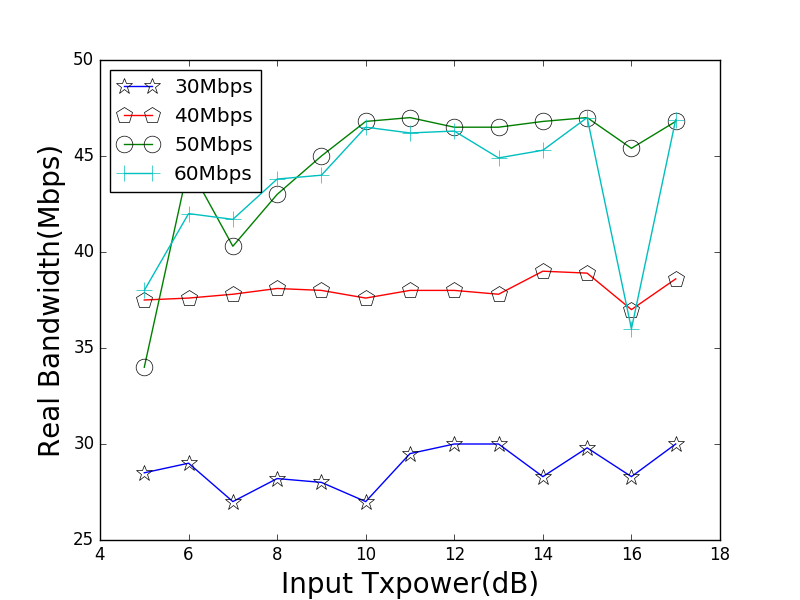
\includegraphics[height=5cm]{hiddenterminal-txpower}}
  \hspace{1em}
  \subcaptionbox{隐藏终端带宽测试实验结果(增加发送功率作为因变量)\label{fig:hiddenterminal-6}}
    {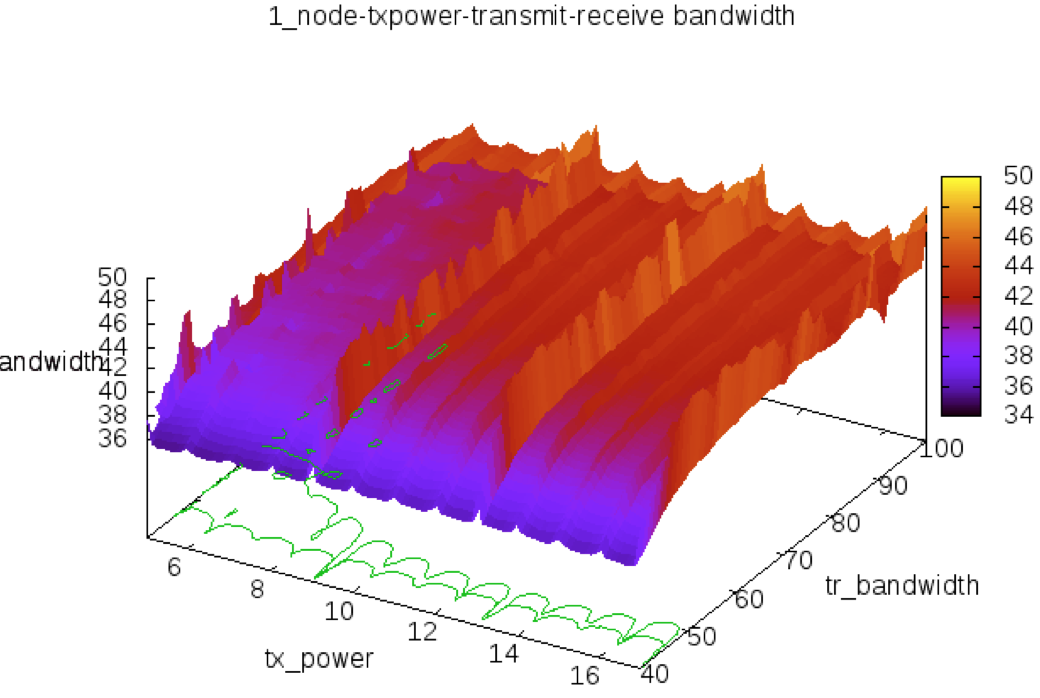
\includegraphics[height=4cm]{hiddenterminal-rts-comp-3d}}
  \caption{引入发送功率的带宽测试结果}
\end{figure}

\subsection{子网划分与信道分配}
由上述实验可以看出相邻链路干扰和隐终端的存在会给Mesh网络的实际有效带宽带来很大的干扰。
因此在进行总体网络规划的时候,选择进行子网划分,子网内部工作在同一信道,子网之间
采用正交信道,避免相互干扰。

5GHz在高频段有10个可用信道(根据所在国家和地区有差异)。设置20Mbps的信道宽度,则可以划分为
5个互相正交的独立信道。根据四色定理,平面空间中的区块可以用四种颜色着色,相邻区块不会出现
重色。据此,我们将整个网络划分为多个相邻的子网。子网内部独立自组织形成Mesh网络,每个子网
选择一个节点作为簇首节点,簇首节点作为该子网联通外部网络的网关。上层簇首节点因为数量
可控,我们通过桥接形式接入远距离定向无线传输设备。这样最终的网络架构将是一种两层结构。
该结构既保留了Mesh网络的独特优势,又进一步通过分层分信道划分子网,达到隔离干扰域,优化
整体网络吞吐量的目的。

划分子网的另一个好处是,在我们的系统目标场景中,油田是一个重要的应用场景,而在野外的油田
分布十分分散,一套Mesh网络形成大范围覆盖效果并不理想,并且会需要大量的中继节点,
造成严重的资源浪费。为此我们可以在每一个油田或相邻的几个油田部署独立的一套
Mesh子网,完成对该油田区域的覆盖,可以提供充足的带宽用于监控、生产数据的传输。最终通过
簇首桥接远距离定向无线设备将数据汇总至油田的控制中心。

基于以上实验,我们搭建了大型的室内实验平台,使用3.1节中介绍的硬件平台配置了101个Mesh
节点。将这101个节点划分为10个Mesh子网,每个Mesh子网的簇首桥接一个远距离无线设备,无线设备
与sink直接通信。实验网络逻辑划分和实际平台分别如图~\ref{fig:subnetexam}如图~\ref{fig:subnet}
所示。因为原硬件平台天线信号覆盖范围最大可达
3~5km,显然会造成整个实验床的全覆盖,形成严重的节点之间的干扰,实验验证在这种情况下视频
完全无法传输。于是我们给天线加装衰减器,通过调节衰减器的衰减性能将天线信号覆盖范围控制在
三米左右。这样可以基本保证划分的子网做到一定的区分。

\begin{figure}[H] % use float package if you want it here
  \centering
  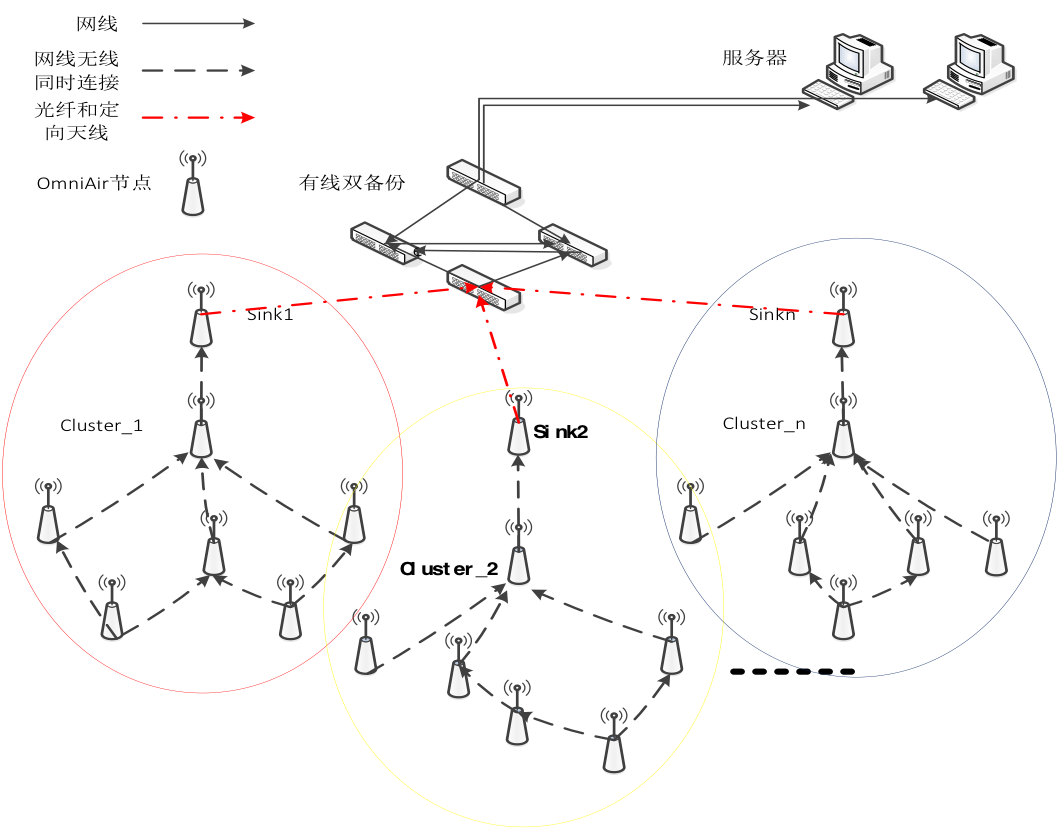
\includegraphics[width=0.6\textwidth]{subnet_exam}
  \caption{子网逻辑划分}
  \label{fig:subnetexam}
\end{figure}
\begin{figure}[H] % use float package if you want it here
  \centering
  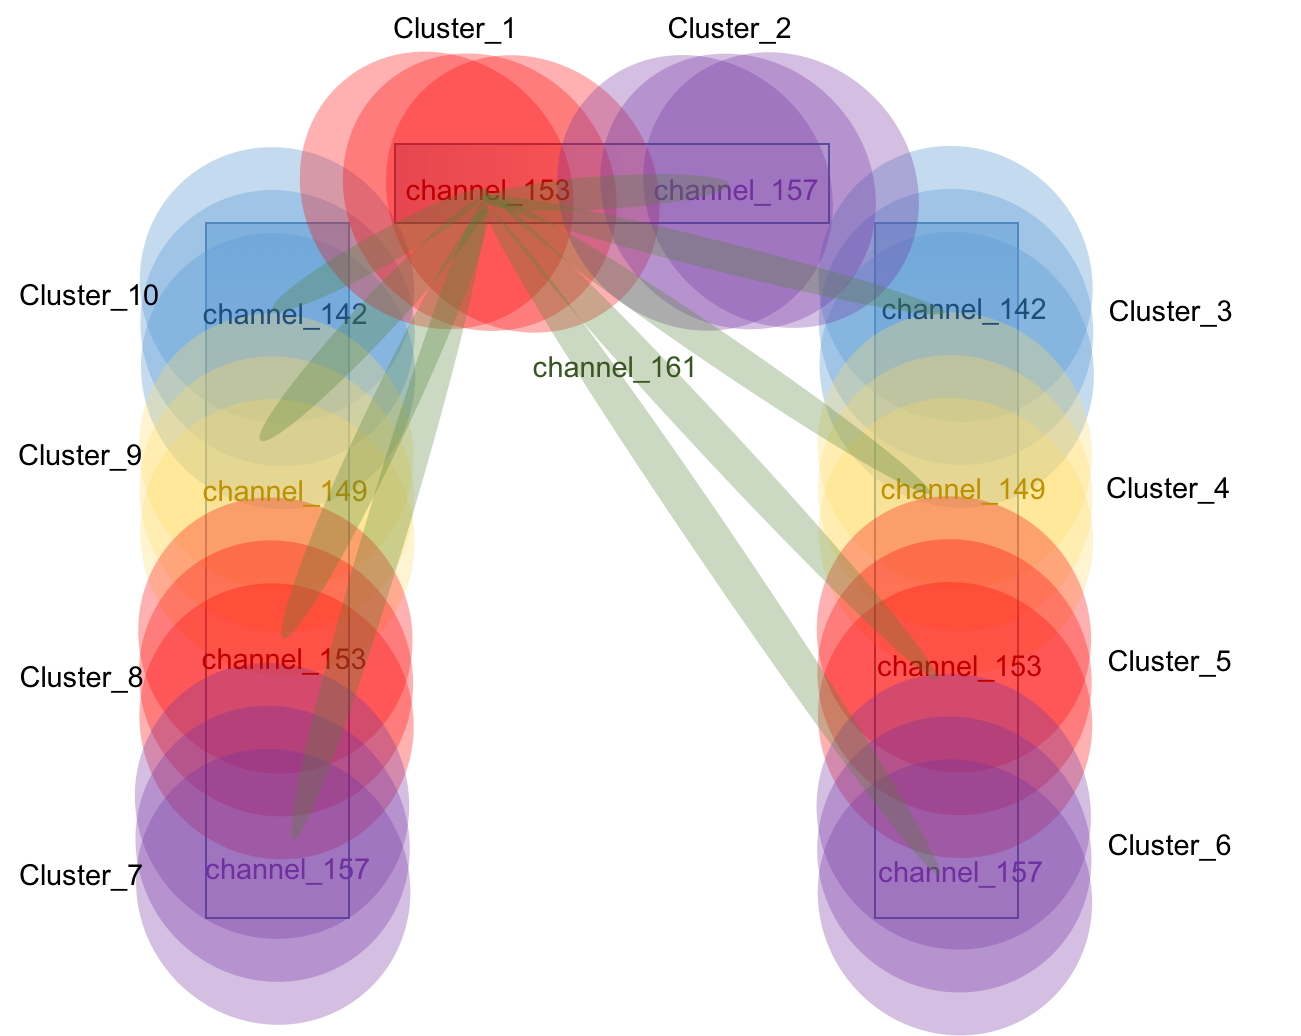
\includegraphics[width=0.5\textwidth]{Subnet-interference}
  \caption{子网间干扰示意图}
  \label{fig:subnet_interference}
\end{figure}
\begin{figure}[h]
  \centering
  \subcaptionbox{}
      {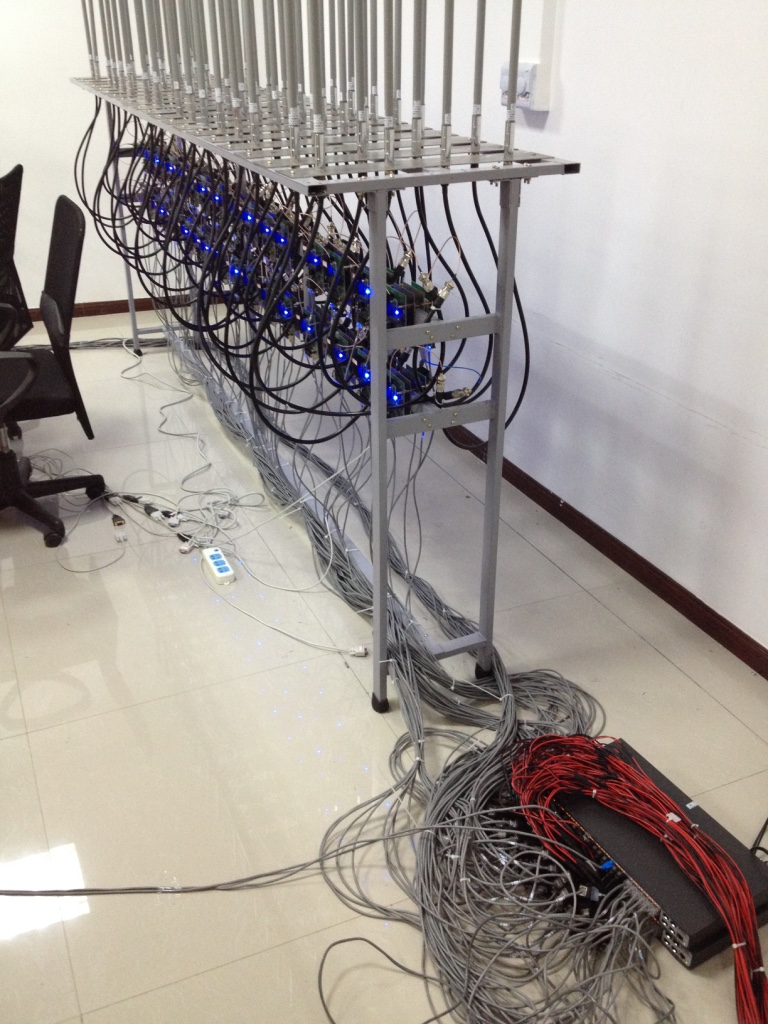
\includegraphics[height=5cm]{Subnet-3}}
  \hspace{1em}
  \subcaptionbox{}
    {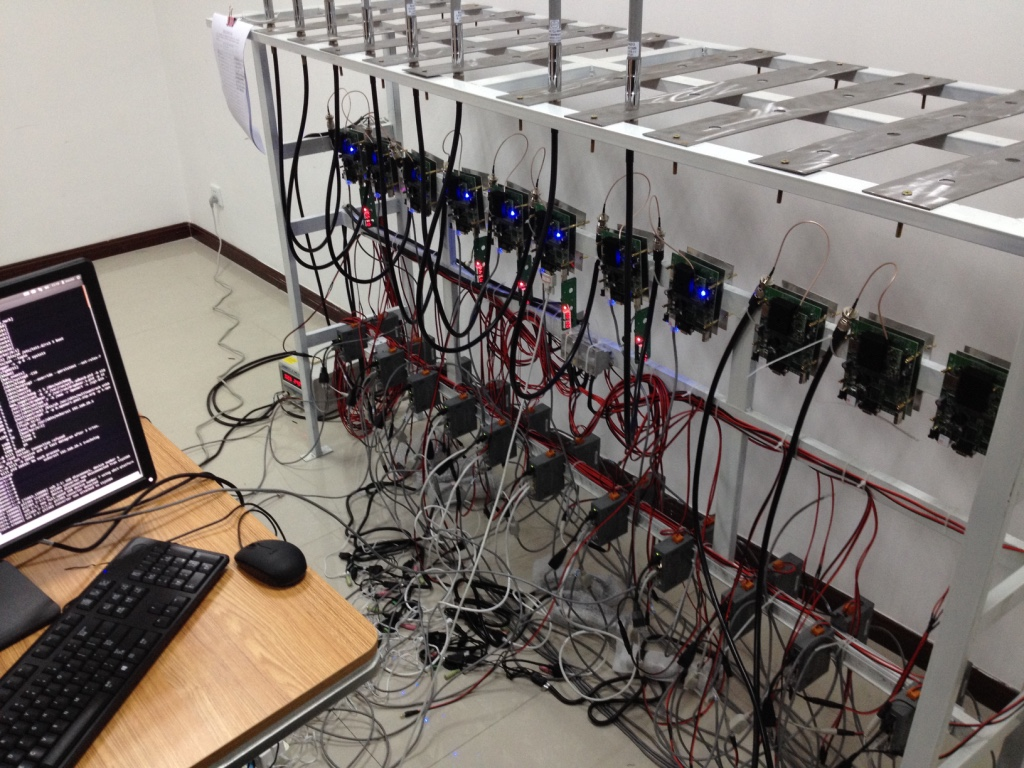
\includegraphics[height=4cm]{Subnet-1}}
  \hspace{1em}
  \subcaptionbox{}
    {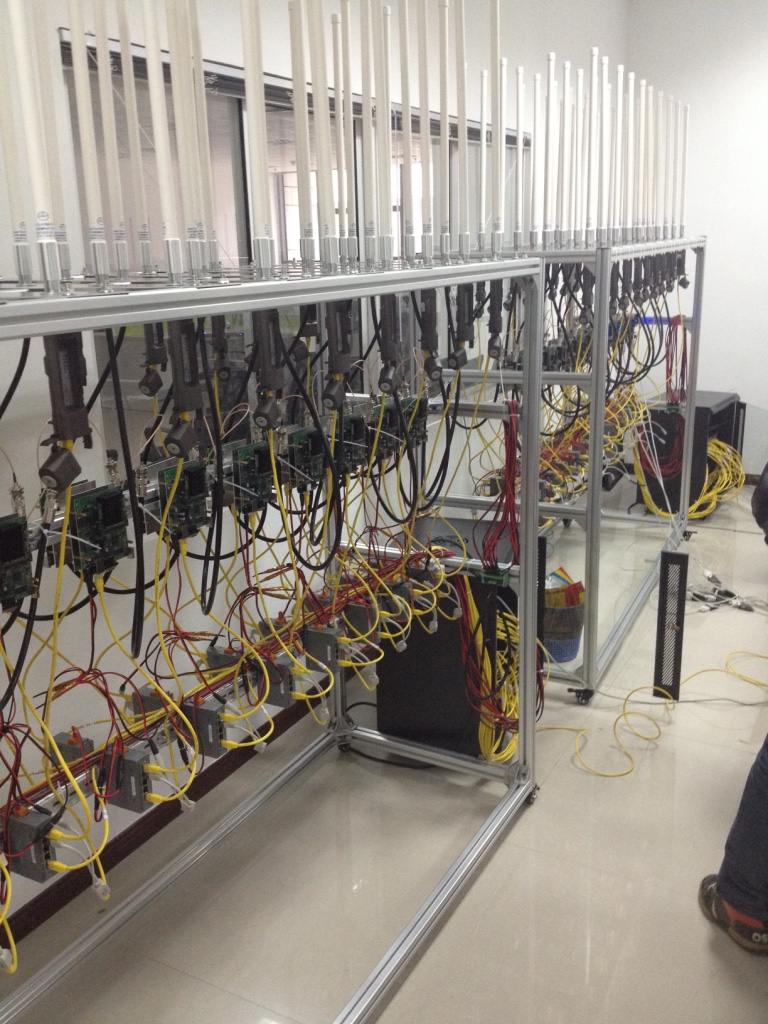
\includegraphics[height=5cm]{Subnet-2}}
  \caption{子网划分实验床}
  \label{fig:subnet}
\end{figure}

实验床的节点物理位置及干扰分布如图~\ref{fig:subnet_interference}所示,图中每种颜色代表一个独立的信道,
相互正交,相邻信道间隔为两个独立信道,因此不存在干扰。图中蓝、黄、红、紫分别代表5GHz频段
的142、149、153、157号信道,这四个信道用于分配给子网,根据四色定理,存在这样的方案使得
任意相邻信道之间不存在干扰。因为不同子网间节点在不同信道,互相之间不可见,因此组网协议在不同
子网间也是不可组网的,这样就实现了子网的隔离,而子网内部可以自由组网。

这样的子网是
相互独立的,而我们最终需要的是一个整体的网路,因此我们使用两层架构,在子网之上,每个子网的簇首
节点桥接一个上层节点,该节点采用定向发送方式,因此虽然需要更高的传输功率但干扰范围可控,
且独立占据一个与所有子网都不相互干扰的信道。

完成配置部署后我们进行了实验验证,该方案带来的性能提升十分巨大,如表~\ref{tab:subnet_comp}所示。
实验比较了不同的信道划分方案,主要分两类,一种是所有节点均采用同一信道,全干扰状态下进行视频
传输实验,另一种是上述子网划分方案。在第一种单一信道实验中,用三种不同且相互正交的信道分别
进行,以排除环境中可能的信号干扰。在每个子网中接入3路视频,一共30路视频,每一路视频占用传输
带宽设置为2Mbps。实验结果以实际视频的传输质量为参照。后期进一步的实验显示实验
网络最大的承载量为200路高清摄像头的数据,约为400Mbps的实时数据流。

从表~\ref{tab:subnet_comp}中显而易见,子网划分方案带来的性能提升是显著的,单一信道在这样的
全干扰状态下几乎无法正常工作。
\begin{table}[htbp]
  \centering
  \caption{子网划分性能提升对比}
  \label{tab:subnet_comp}
  \begin{tabular}{|c|c|c|}
  \hline
  信道方案 & 实际效果 \\
  \hline
  单一信道方案(142信道) & 簇1内三路视频可见,簇2、簇3各一路视频可见 \\
  \hline
  单一信道方案(149信道) & 仅簇1内一路视频可见 \\
  \hline
  单一信道方案(153信道) & 仅簇1内一路视频可见,其他簇偶尔出现断断续续的视频 \\
  \hline
  子网划分方案 & 所有视频均可见,偶尔会出现卡顿现象 \\
  \hline
  \end{tabular}
\end{table}

\section{跨层视频帧权重差分}
\label{sec:2}
在过去的二十多年中,无线局域网中的视频流传输研究吸引了大量的研究人员的努力,其中很多的工作
都聚焦在QoS管理方面。比如,802.11e定义的EDCA,在mac层实现了不同的权重队列,每个队列对应
不同的发送优先级,上层过来的业务数据根据类型被映射到不同的权重队列中。视频和音频数据通常
具有更高的机会进入高优先级的发送队列。相对于传统的802.11的信道竞争机制,EDCA的支持
下,视频音频数据将获得更好的传输带宽,从而带来更好的用户体验。

另一方面,视频帧编码技术将视频编码为不同权重的帧,权重更高的帧对于视频的解析更重要,甚至
仅有高权重帧的情况下,也可以解码出流畅但不甚清晰的视频。由此,将视频帧帧解码为不同权重
的帧映射到不同的EDCA权重队列中,就可以实现在带宽资源匮乏的情况下,优先传输高权重
视频帧的目的。

目前,一些研究工作已经将这一想法引入了无线Mesh网络,但是并没有取得显著的效果。特别是在
网络规模扩大或者视频数据量增大的情况下,带宽很容易耗尽~\cite{Iptvhome}。
其他研究工作提出网络中的在线
视频数据削减~\cite{W4}。但是,计算机视觉技术会需要很大的资源开销,这对计算资源受限的mesh节点是一个
极大的挑战。另一方面,相关工作大多数都是通过仿真软件来完成,缺少实际系统的验证。

通过细致的实验分析,我们发现现阶段很多工作提出的映射机制和入队算法越来越复杂化,能够优化
的空间越发有限。一个可能的性能突破的方向是对数据进行更加细粒度的分析。例如对于视频数据帧,
不仅仅停留在编码帧的层面,而是深入观察相同的编码帧之间的差异,达到更好的映射效果。该想法
基于我们实验中的三点发现:
\begin{itemize}
\item[1.] 属于同一类型的编码帧在解码过程中的权重不同。典型的视频帧编码标准比如H.264和MEPG-4
将视频帧编码为三种不同类型的帧,分别是I帧、P帧和B帧。实验发现,属于统一个组的P帧权重依次递减,
B帧也呈现同样的规律。
\item[2.] 因为同一个编码帧可能在网络层或者更低层被分割为不同的数据包,这些数据包同样会呈现
不同的重要性。因此,在设计映射机制的时候,应该深入不同该层次的数据包,而不是停留在编码帧的
层面。
\item[3.] 映射机制应该具有足够的灵活性,使不同类型的编码帧都有机会使用高权重的发送队列,
最大限度的利用有限的带宽。
\end{itemize}

基于以上,本项目提出一种无线Mesh网络视频帧的mac层权重队列映射机制,全面的考虑了编码帧类型
、帧出现的位置、更细粒度的数据包形成最终的映射方案。该方案可以在高效的网络传输和有限的节点
计算资源之间做到很好的平衡。

\subsection{视频帧分层编码}
视频数据一直是数据量最大的业务数据类型,再如今大数据火热的阶段,尤其被关注,在无线网络中
视频数据同样也给网络传输带来了极大的挑战。不同的视频编码技术应运而生,在这之中,H.264和
MPEG-4被业界广泛接收和使用。这种类型的编码方式在性能和编码复杂度上都能够很好的满足大多数的
应用场景。

分层编码技术将视频编码为三种不同类型的帧:I帧、P帧、B帧。每一种帧在视频解码时都扮演不同的
角色。
\begin{itemize}
\item I帧(帧间编码):该帧数量最少,包含全部用来解码其自身的信息,这就意味着I帧的解码不需要
依赖其他I帧或者P帧、B帧。I帧通常压缩为一个静态图像,体态也较P帧、B帧更大。
\item P帧(前向预测帧):该帧包含它之前最近的I帧和P帧之间的差异,因此需要依赖之前的I帧和P帧来
解码。
\item B帧(双向预测帧):该帧压缩尺度最大,需要依赖其之前和之后的I帧和P帧来解码。
\end{itemize}

\begin{figure}[H] % use float package if you want it here
  \centering
  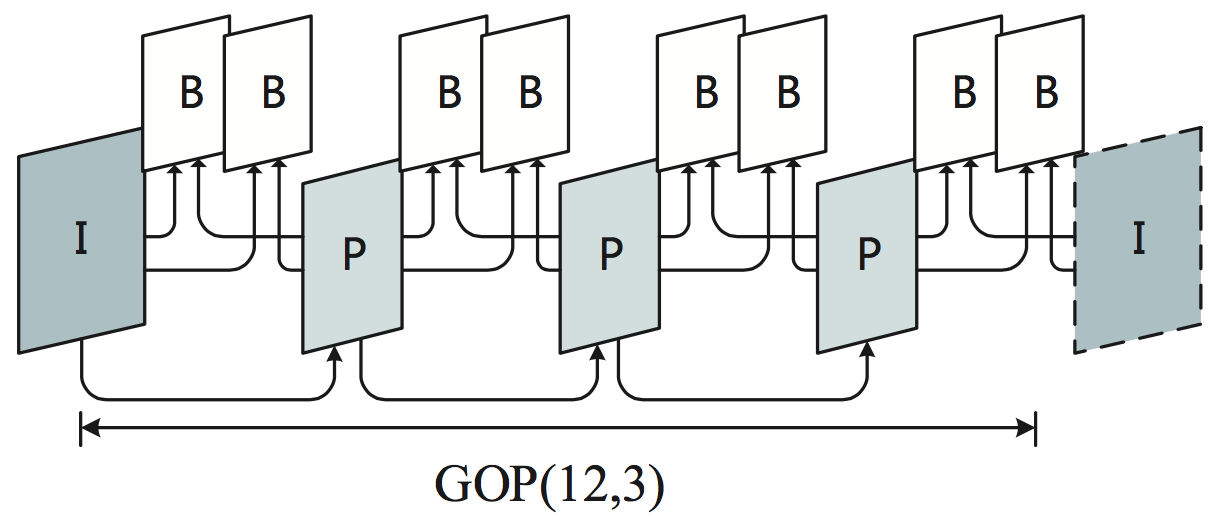
\includegraphics[width=0.6\textwidth]{GOP}
  \caption{GOP结构示例,GOP(12,3)}
  \label{fig:gop}
\end{figure}
根据H.264和MPEG-4编码,一小段视频会被解析编码为一组重新组织过的帧,这一组帧称为GOP。每个
GOP总是由一个I帧开始,之后跟随一段连续的P帧和B帧。GOP的结构可以表示为两个参数G(N,M),其中
N表示GOP中包含的所有帧的数量(两个连续I帧之间的距离),M表示I帧和其后第一个P帧之间(
或者两个连续P帧之间)的距离。图~\ref{fig:gop}为G(12,3)的结构示例,分解后即为:‘IBBPBBPBBPBB’。

如图~\ref{fig:gop}所示,GOP内部的不同帧之间紧密相连,不同的GOP之间相互独立。实质上,I帧不
依赖于任何其他帧,可以单独解码,P帧依赖于其之前的I帧或者P帧,B帧依赖于其前后的I帧或者P帧。
也就是说,如果在传输过程中,丢失了I帧则整个GOP都无法解析。类似的如果一个P帧丢失,则其后
的P帧和B帧均无法解码。而B帧丢失仅影响其自身,其他数据帧不会收到任何影响。由此我们可以总结
三种类型帧的重要性,显然I帧>P帧>B帧。

综上,处于QoS保障的考虑,当带宽紧缺时,需要保证重要性更高的帧优先传输。

\subsection{802.11e增强分布式协调访问(EDCA)}
传统的IEEE802.11标准分布式信道接入协调功能(DCA)做为基础的信道接入方式,该方式基于CSMA/CA,
不提供QoS保障。为了支持区分的服务,802.11e引入了一种混合协调功能(HCF),其中包含两种并行
机制:混合控制信道访问(HCCA)和增强分布式协调访问(EDCA)。本项目中基于EDCA功能展开。

EDCA通过引入四个不同的接入类型(AC)来提供QoS保障。传统的802.11信道接入方式维护一个发送队列,所有
业务数据平等的进行信道竞争,不同于此,每个AC的数据维护各自的发送队列,通过竞争窗口控制
每个队列竞争获得信道的概率不同。如图~\ref{fig:acofedca}所示,四个队列按权重从低到高依次是:
AC\_BK(背景数据),AC\_BE(尽最大努力传送),AC\_VI(视频),AC\_VO(声音),依次编号为AC(0),AC(1),
AC(2),AC(3)。不同的权重通过设置不同的信道竞争参数实现,包括竞争窗口界限、仲裁帧间隔、
发送机会限制。

默认情况下,QoS支持在EDCA中的实现是通过将实时数据包括音频视频映射到AC(2)和AC(3)中,其他的
数据则映射到AC(0)和AC(1)。EDCA机制不考虑视频帧的不同类型之间重要性的区别,将所有的编码都
映射到AC(2)中。然而,在视频监控的场景中,除了少量的控制数据,几乎所有的数据都是视频数据,
这些数据都被映射到同一队列,很容易造成该队列的饱和,进一步造成丢包,影响传输质量。因此,在
无线Mesh网络中,尤其在视频流作为主要传输数据的场景中,应该充分挖掘视频帧编码之间的差异,
利用EDCA四个队列的功能来实现更好的用户观看体验。之前已经有一些工作做过这方面的尝试,图
~\ref{fig:originmapping}给出了静态映射和动态映射的对比。静态映射,比如~\cite{staticmapping}
,仅仅将不同重要性的帧固定的放入固定的队列,这样会造成优先队列资源的浪费。动态映射,比如
~\cite{dynamicmapping},进一步考虑
网络地动态状况和队列地占用情况,动态地进行队列映射,提高了网络地利用度。

\begin{figure}[H] % use float package if you want it here
  \centering
  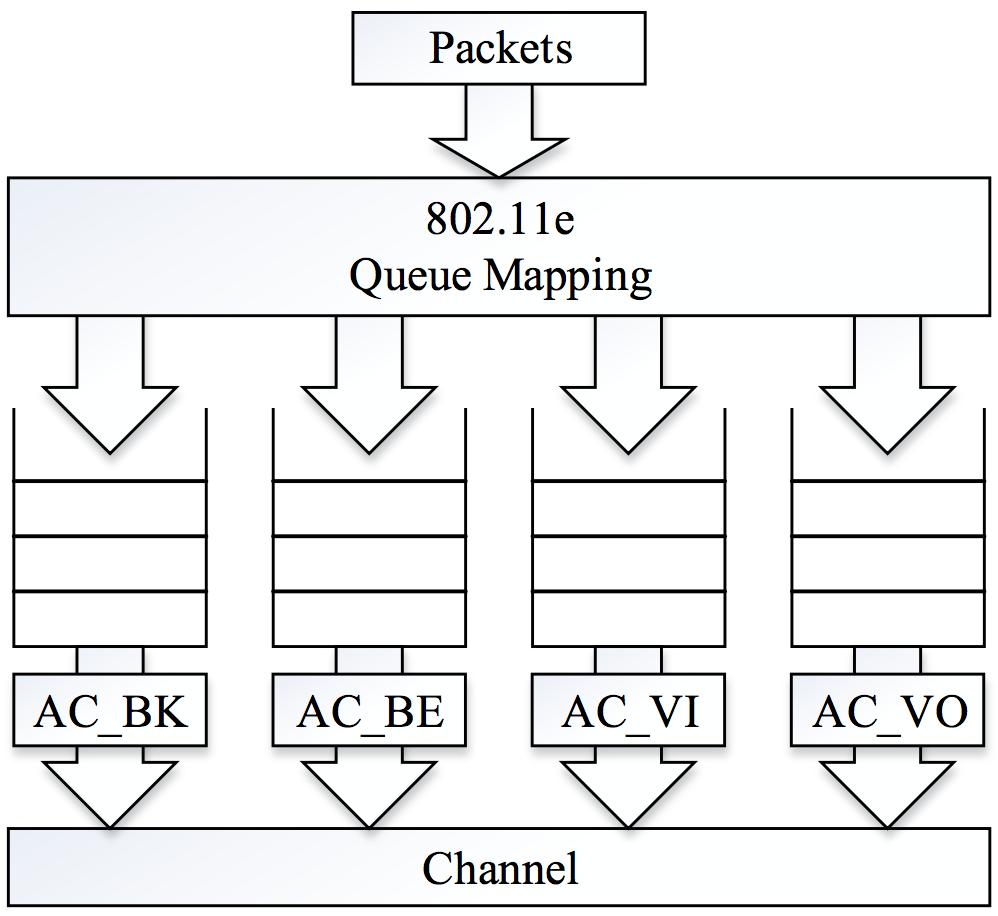
\includegraphics[width=0.5\textwidth]{ACofEDCA}
  \caption{EDCA的四个AC队列}
  \label{fig:acofedca}
\end{figure}
\begin{figure}[H] % use float package if you want it here
  \centering
  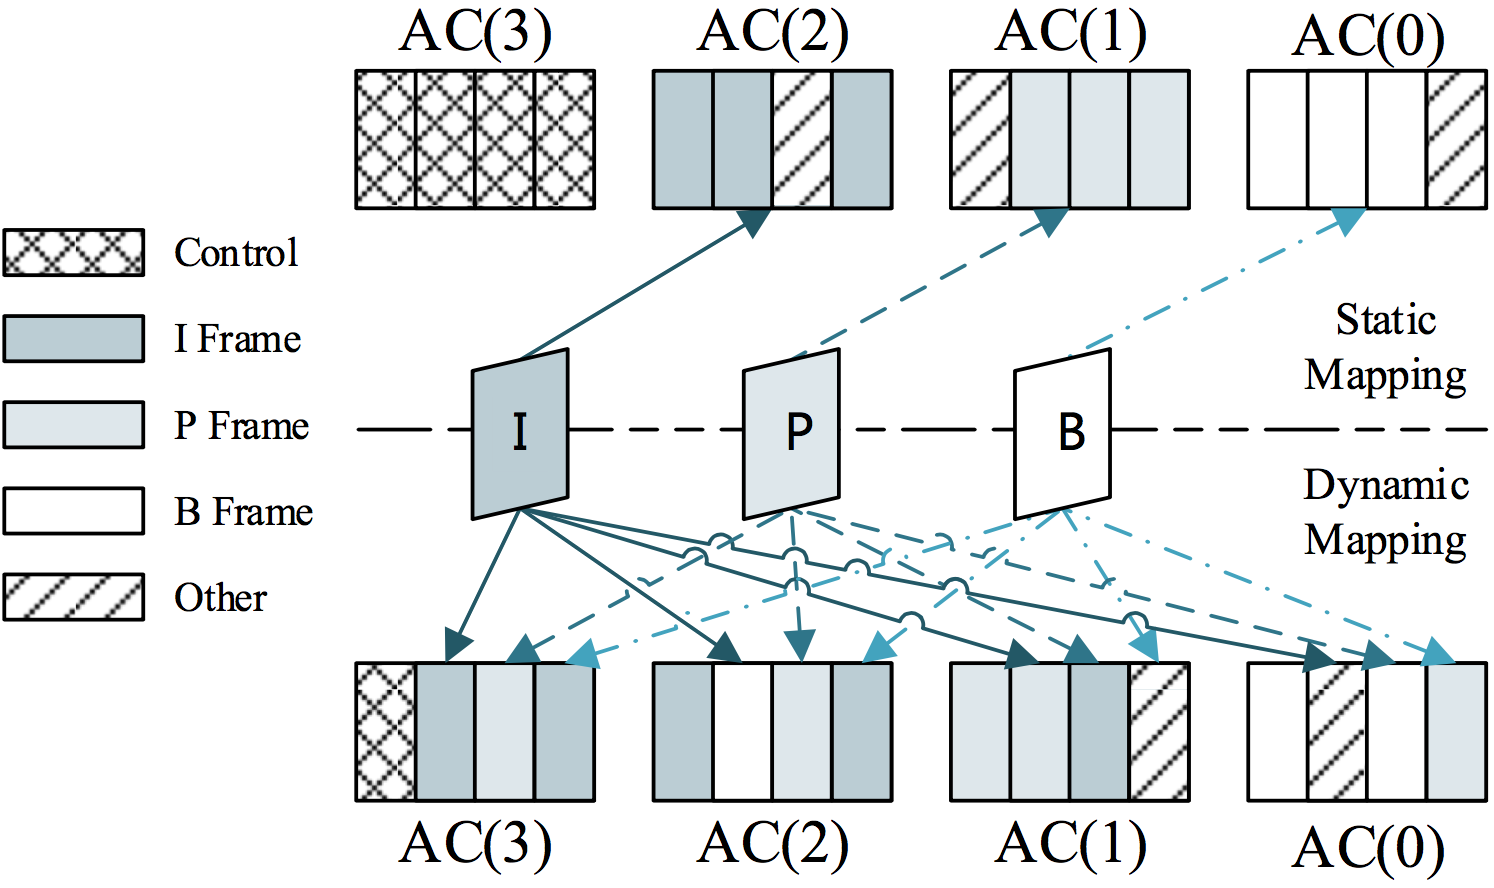
\includegraphics[width=0.6\textwidth]{mapping}
  \caption{静态映射和动态映射机制示例}
  \label{fig:originmapping}
\end{figure}

\subsection{视频帧映射机制}
基于GOP编码结构和EDCA机制,结合细粒度地分析视频数据包,我们提出了一种跨层映射方案,实验显示该
所提方案相对于朴素地基于EDCA传输方案,优化效果>50\%。

在视频监控系统中,视频数据占所传输带宽的绝大部分。在衡量视频传输质量的时候,除了传统网络
度量参数如丢包率等,更重要的是视频观看体验,目前普遍使用的衡量指标是峰值信噪比(PSNR)和结构
相似性指标(SSIM)。视频传输的流畅、实时、清晰是视频监控系统的首要目标。

受通用视频编码技术中的分层编码的影响,可以认为不同类型的帧对视频的传输质量贡献不同。这是由
分层编码中GOP内部不同帧之间的依赖关系决定的。如前所述,I帧独立于其他帧,可独立解码
其压缩率也最低;P帧依赖于其之前的I帧或者P帧,压缩率次之;B帧压缩率最高,但需要依赖其前后的
I帧或者P帧来解码。不难发现,I帧丢失则该GOP内全部的帧都无法解码;P帧丢失则其后的所有帧无法
解码,B帧丢失则仅其自身无法解码,不影响其他帧。

\begin{figure}[h]
  \centering
  \subcaptionbox{}
      {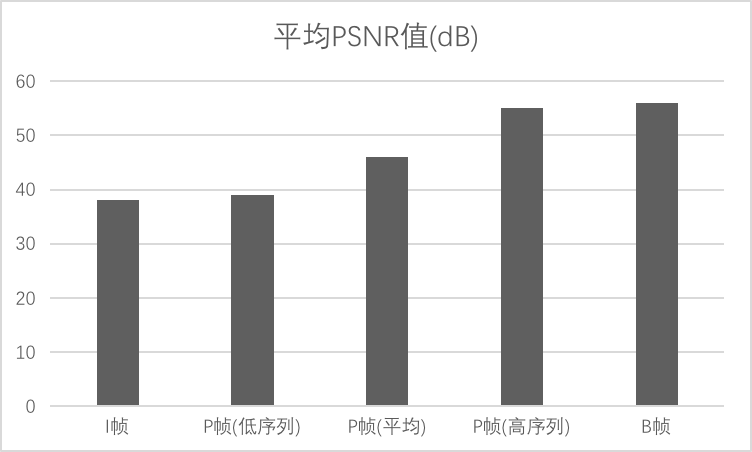
\includegraphics[height=4cm]{Ave_PSNR}}
  \hspace{1em}
  \subcaptionbox{}
    {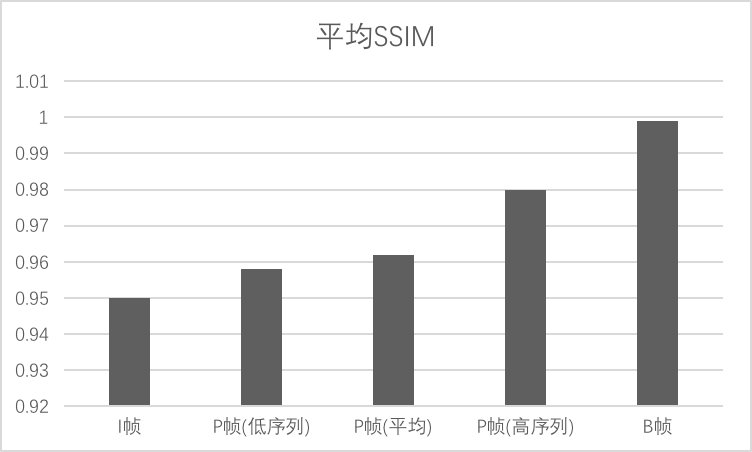
\includegraphics[height=4cm]{Ave_SSIM}}
  \caption{I帧、P帧、B帧丢失对视频质量的影响比较}
  \label{fig:ipb-comp}
\end{figure}

\begin{figure}[h]
  \centering
  \subcaptionbox{}
      {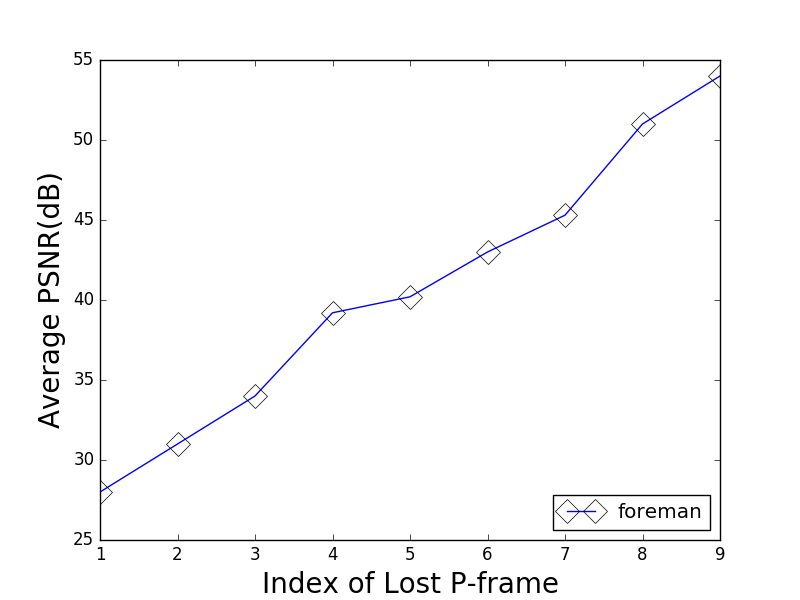
\includegraphics[height=5.3cm]{Position-comp1}}
  \hspace{1em}
  \subcaptionbox{}
    {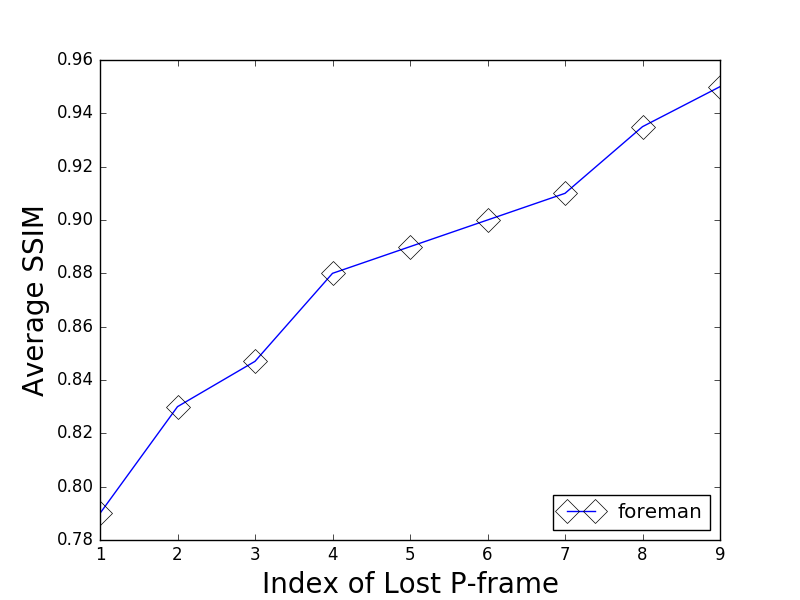
\includegraphics[height=5.3cm]{Position-comp2}}
  \caption{不同位置的P帧丢失对视频质量的影响比较}
  \label{fig:position-comp}
\end{figure}

图~\ref{fig:ipb-comp}和图~\ref{fig:position-comp}
给出了I帧、P帧、B帧以及同一个GOP中不同位置的P帧丢失对视频质量的影响。可以看出,和我们预测
的相同,在相同的数量上,I帧对视频质量的贡献明显大于P帧,P帧中出现在靠前位置的P帧影响力
又要大于之后的P帧,而B帧对视频质量的影响最小。

之前的关于映射机制的工作,仅仅按照编码帧的类型进行映射,而没有考虑不同位置帧的重要性不同。
我们将这一点引入映射机制,综合考虑帧的\emph{类型}和\emph{位置}。下面详细介绍该映射机制的
细节原理和实现。其中核心分为两部分,帧权重计算和帧映射。

\begin{table}[htbp]
  \centering
  \caption{本章符号检索}
  \label{tab:notations}
  \begin{tabular}{p{3cm}p{8cm}}
  \hline
  符号 & 意义 \\
  \hline
  N, M &  GOP参数 \\
  $\omega$ &  数据包权重值 \\
  $f_{0}$ & 受当前帧影响的帧数量 \\
  $f_{1}$ & 影响当前帧的帧数量 \\
  $\alpha$, a, b & 权重值计算公式参数 \\
  $b_{0}$ & 权重值基线 \\
  h & 帧分解的第一个数据包的额外权重 \\
  p & P帧在GOP中的位置索引 \\
  \emph{threshold(i)} & AC(\emph(i))的最大队列缓存 \\
  \emph{qlen(i)} & AC(\emph(i))当前使用长度 \\
  \hline
  \end{tabular}
\end{table}

\renewcommand{\thesubsubsection}{\Alph{subsubsection}.}
\subsubsection{权重计算}
对于I帧,因为其相对于P帧和B帧数量极少,且对于解码GOP起到至关重要的作用,所以在权重上赋最
大值1,即为$\omega =1$;对于P帧和B帧,它们的重要性和它们之前的需要依赖的帧以及它们后续的
依赖于它们的帧有关。这里我们定义受当前帧影响的帧数量为$f_{0}$,对当前帧有影响的帧数量
为$f_{1}$。进一步的定义当前帧的权重计算公式为:
\begin{equation}
\omega = g(f_{0}\alpha^{f_{1}})
\end{equation}
在这里,$\alpha \in (0,1)$是一个权重常量,用来平衡$f_{0}$和$f_{1}$,$f_{0}\geq1$(所有的P
帧和B帧至少被I帧影响),$f_{1}\geq1$(每一个帧至少影响它本身),g(x)是一个单调递增函数。
这就意味着,越多的帧依赖于当前帧,或依赖于当前帧的帧越少,则当前帧的权重就越高。更直观
的讲,就是在一个GOP中出现越早的帧相对于晚出现的帧权重更高。

g(x)定义为:
\begin{equation}
g(x) = a(\log (x) + b) + b_{0}
\end{equation}

带入$\omega$表达式则有P帧和B帧数据包的权重值计算公式:
\begin{equation}
\label{equ:omega}
\omega = a(\log f_{0} + f_{1}\log \alpha + b) + b_{0}
\end{equation}

上式中,$b_{0}$是作为权重值的基线,确保B帧能够有机会进入优先级较高的队列。a、b和$b_{0}$
用来限制$\omega$在[$b_{0}$,1]的范围内,a,b值定义为:
\begin{equation}
a = \frac{1-b_{0}}{\log(N) - \log(\alpha^{N/M})},
b = -\log(\alpha^{N/M})
\end{equation}

上式中,$\log(N)$和$\log(\alpha^{N/M})$分别为$\log(f_{0}\alpha^f_{1})$的最大值和最小值。
对于一个GOP中的第\emph{p}(\emph{p}>0)个P帧,$f_{0}=N+M-1-M*p$, $f_{1}=p$。对于任意第
\emph{p}个P帧后的B帧,有$f_{0}=1, f_{1}=2$。

目前为止,我们定义了普通的视频帧数据包的权重计算方法,该方法充分利用GOP结构中不同\emph{类型}
帧不同的重要性。下面我们考虑利用同\emph{类型}不同\emph{位置}帧重要性不同的性质,其中关键
的是一个视频帧被底层协议拆分为一个个的数据包时,最重要的是第一个数据包,其中包含了编码重要
的信息。我们选择添加一个额外的值\emph{h}来提升第一个数据包的权重。如果出现$\omega+h>1$,就设置
$\omega=0.99$。之所以这里不设$\omega$为1是考虑到防止P帧或者B帧抢占I帧的优先权,在保证I帧
绝对优先权的基础上最大限度提升P帧或者B帧较重要的数据包的传输几率。

\subsubsection{帧映射}
所谓帧映射就是将计算得到的不同权重的帧的数据包映射到不同的EDCA的AC中,区分他们在发送时的优先权。
根据上一节涉及的权重计算方法,可以计算出每一个视频帧对应的权重值,帧映射即根据该权重值
完成。映射的直接原则是充分使用高权重队列以降低传输延迟和丢包率。当网络质量良好,传输数据量
较小时,甚至可以将B帧映射到AC(3)中,所有帧都可以以最低延迟,最高的优先权完成传输。相反,
当网络质量较差,网络传输数据量过大,造成拥堵时,映射机制优先将I帧映射到最高优先权队列,保证
I帧的传输质量。

当一个数据包到达时,映射机制将顺序从最高优先权队列AC(3)开始依次检测。如果发现当前AC有足够的
缓冲区余量,且满足映射标准,即将数据包插入该AC中。判定的标准为,给定一个数据包的权重假设
为$\omega$,如果$\omega*threshold(i)>qlen(i)$,就将数据包插入队列AC(\emph{i});否则,继续
检查优先权次之的队列。其中,$threshold(i)$和$qlen(i)$是AC(\emph{i})可以通过底层API读取的
最大队列长度和当前队列占用。如果一个数据包不能够插入AC(3),AC(2)和AC(1),那么就直接插入AC(0)
而不需要进行进一步的检查。映射算法尽可能设计的简单以减少Mesh节点的计算开销,因为在工业应用
中,Mesh节点能源和计算资源都比较稀缺。

上面的队列映射策略给予了更高权重的数据包更高的概率插入高优先级队列,同时阻止低权重的数据包
阻塞队列。

\subsubsection{映射系统实现}
队列映射如图~\ref{fig:workingflow}所示,跨层架构设计也在图~\ref{fig:crosslayer}中展示。
在结构设计上,因为BATMAN-adv协议主要工作在mac层,且EDCA的四个AC也在mac层实现,所以我们的
权重计算和映射模块均在mac层实现。尽管如此,我们需要考虑来自应用层的数据,网络层的ToS字段,
以及物理层的队列大小及占用情况。实际系统中,每个视频帧的数据包,其权重均在产生该数据包的
第一个Mesh节点计算。当一个Mesh节点接到请求需要发送视频数据时,首先解构GOP为I帧、P帧和B帧,
然后将各个帧在网络层封装为较小的数据包,之后就根据每个数据包所属帧的类型、位置和数据包是否
为帧的头数据包等计算数据包的权重。之后数据包的权重值一值维护在数据包中,在网络传输的过程中
不会改变该权重值。实现中,我们将权重值存储在网络层包头的ToS字段中。

数据包传输到网络中间任一节点时,该节点队列映射也按如图~\ref{fig:workingflow}所示进行,
但不需要重新计算权重值,只需要从ToS字段中取的该权重值即可,之后就根据该权重值,将数据包
插入相应的AC中。

\begin{figure}[H] % use float package if you want it here
  \centering
  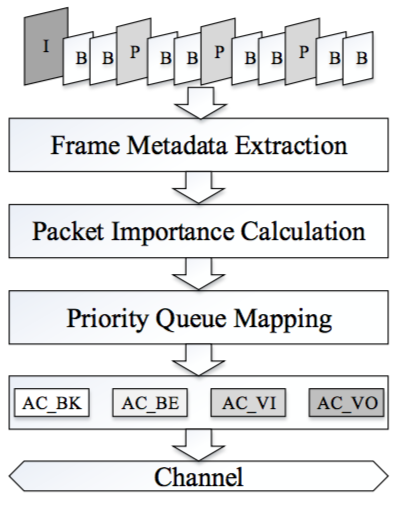
\includegraphics[width=0.4\textwidth]{WorkingFlow}
  \caption{映射机制流程}
  \label{fig:workingflow}
\end{figure}
\begin{figure}[H] % use float package if you want it here
  \centering
  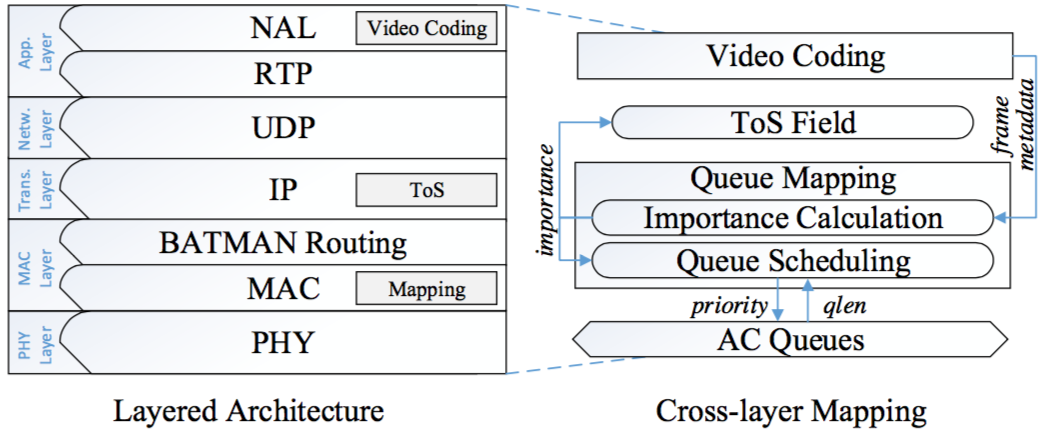
\includegraphics[width=0.8\textwidth]{Crosslayer}
  \caption{映射机制跨层设计}
  \label{fig:crosslayer}
\end{figure}

实验基于室外实际运行的监控网络进行,该系统部署于无锡新区大学科技园清华物联网技术
中心附近,部署图和实验选择的网络拓扑如图~\ref{fig:realdeploy}
\begin{figure}[h]
  \centering
  \subcaptionbox{}
      {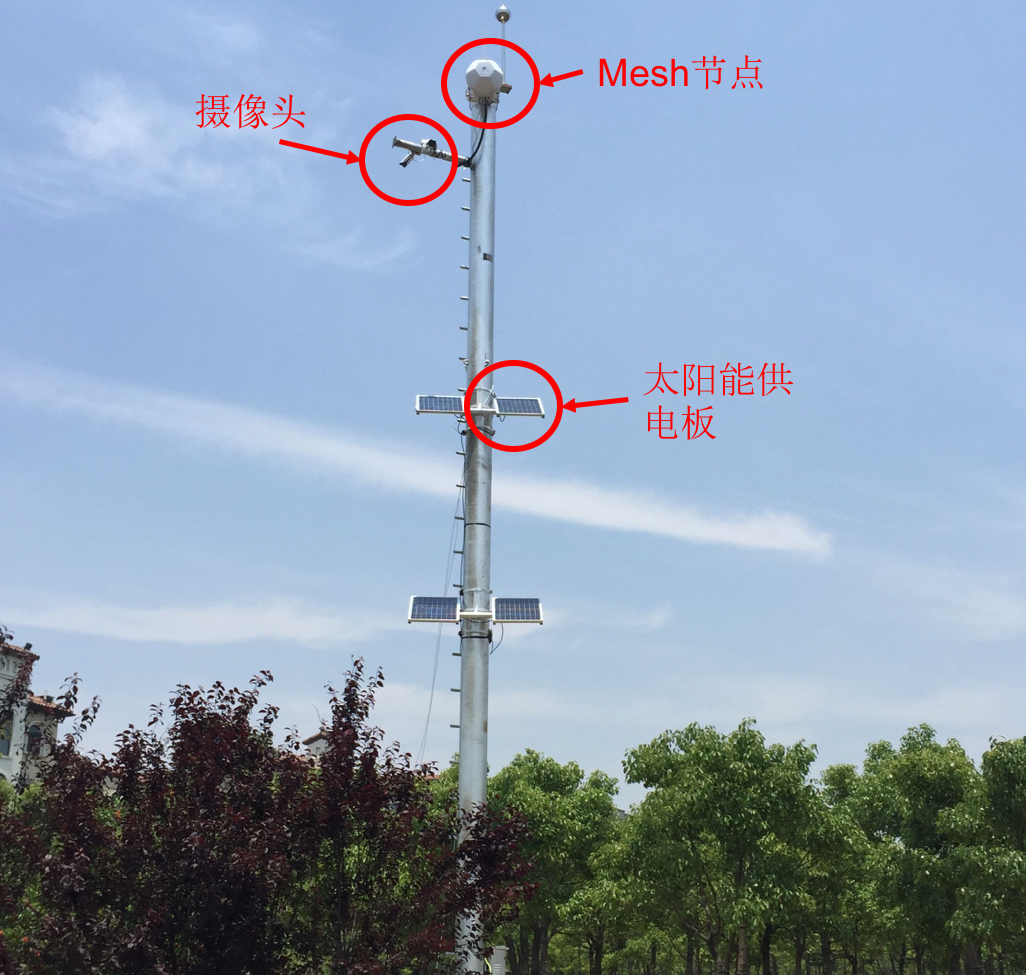
\includegraphics[height=5cm]{realproduct}}
  \hspace{1em}
  \subcaptionbox{}
    {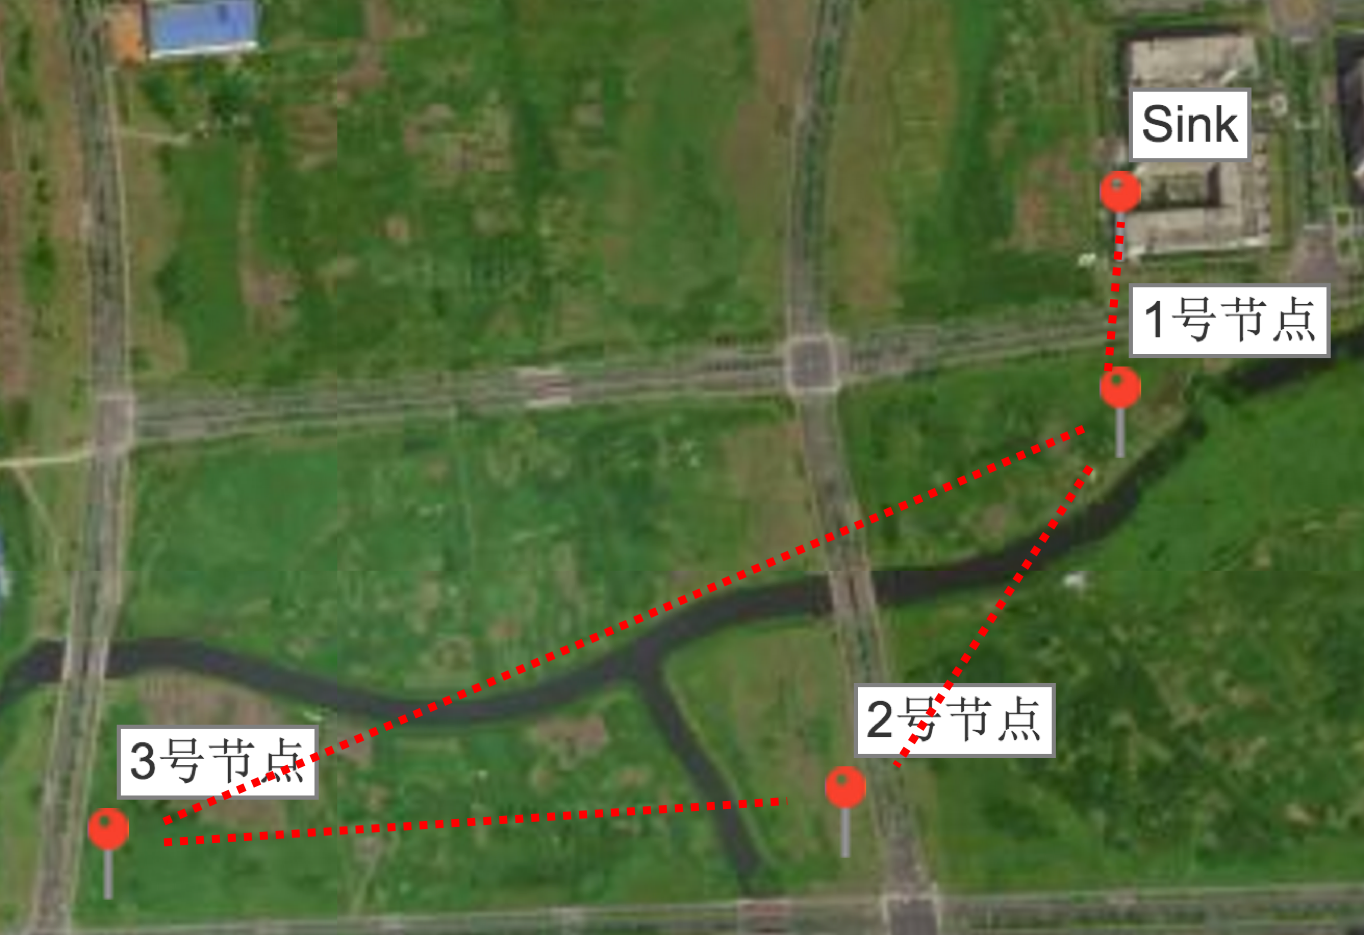
\includegraphics[height=5cm]{deployment}}
  \caption{实际系统部署图示}
  \label{fig:realdeploy}
\end{figure}


\subsection{实验验证}
\renewcommand{\thesubsubsection}{\Alph{subsubsection}.}
\subsubsection{实验方法}
在3.1节已经介绍了项目所采用的软件系统和硬件平台。更细致地,OpenWRT内置的\emph{mac80211}模块
控制数据包的收发。\emph{队列选择}是数据包发送过程中的一个子环节,核心工作就是修改\emph{
队列选择}算法。每当接收到一个数据包,首先检查该数据包包头,如果是一个符合H.264编码标准的
数据包就抓取其中的帧类型、GOP信息和帧编码等。通过公式~\ref{equ:omega}计算出数据包的权重。
之后,根据计算得到的权重值和队列的负荷情况将数据包插入合适的队列中。转发该数据包时,将
权重值记录在IP数据包包头的ToS字段中,之后的转发节点不需要重复计算。

实验中使用公开的视频序列~\cite{videos}中的“foreman”作为基准进行比对。将视频转换为
25帧每秒的GOP(12,3)格式。考虑Mesh延时,将延时超过1秒的视频帧丢弃。

实验中采用的测量参数为PSNR、SSIM和DFR,均为视频图像实验分析常用的标准参数。其中PSNR
描述图像像素级的差异,对于视频则描述视频帧图像差异的平均值;SSIM描述结构差异,更能够
体现人的观看体验。DFR描述解码成功的帧占总帧数的比例,属于帧级别的参数。

我们选取了之前的类似工作做对比。其中SMM~\cite{SMM}基于帧类型;DMM~\cite{DMM}
基于帧类型和流量负载;AMM~\cite{AMM}考虑了帧类型、流量负载和GOP结构;EDCA级802.11默认的映射方法,也即所有视频映射到优先级
次优的队列。

\subsubsection{实验结果及分析}
参数选择上,我们选取参数$\alpha=0.6, b_{0}=0.2, h=0.6$,AC(0)到AC(3)的\emph{threshold}
分别设为$\lbrack\infty, 80, 50, 50\rbrack$。图~\ref{fig:overall_performance}给出了不同映射算法在视频
图像上的直观体现。图~\ref{fig:parameters}给出了PSNR和SSIM两个参数的对比。

\begin{figure}[H] % use float package if you want it here
  \centering
  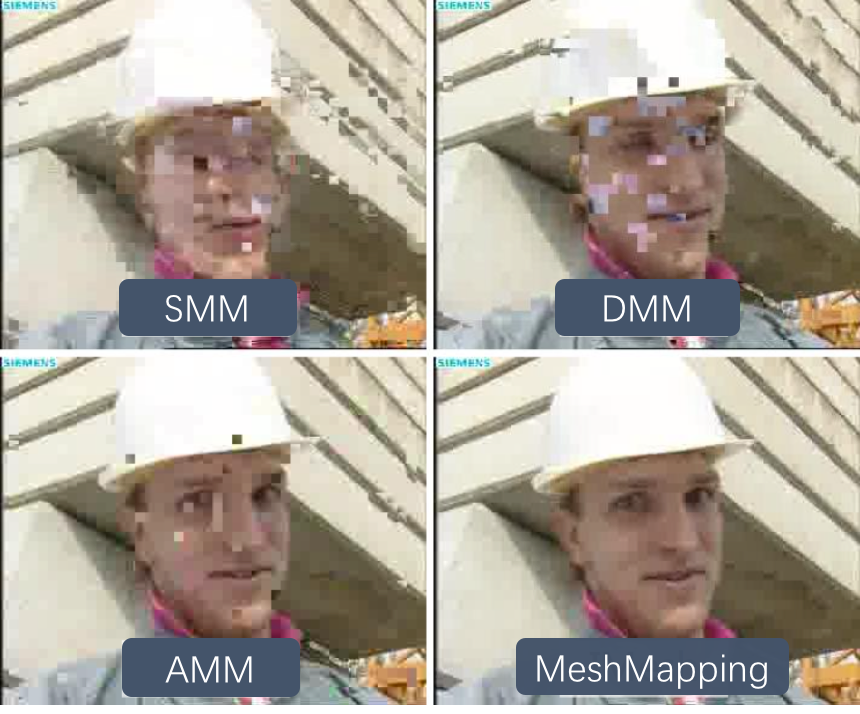
\includegraphics[width=0.5\textwidth]{Overall_performance}
  \caption{映射算法效果比较}
  \label{fig:overall_performance}
\end{figure}

\begin{figure}[h]
  \centering
  \subcaptionbox{}
      {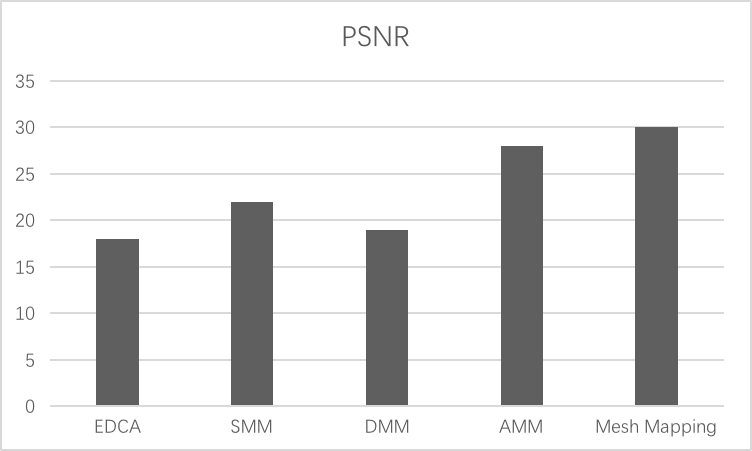
\includegraphics[height=4cm]{PSNR}}
  \hspace{1em}
  \subcaptionbox{}
    {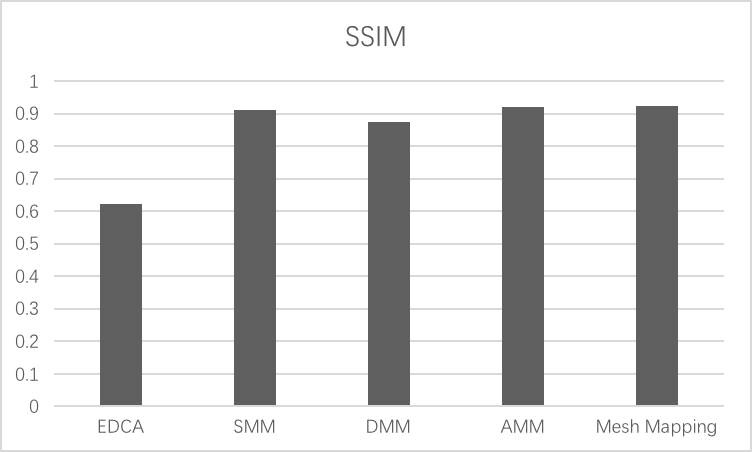
\includegraphics[height=4cm]{SSIM}}
  \caption{映射算法度量参数比较}
  \label{fig:parameters}
\end{figure}

其中MeshMapping即本文所提出的映射算法。可以看到MeshMapping在PSNR参数上要明显优于其他算法,
在SSIM也不弱于其他算法。相对于EDCA更是能够在PSNR和SSIM两个参数上分别优化74\%和54\%。

进一步地,我们研究公式~\ref{equ:omega}中参数对性能的影响,包括$\alpha$, $b_{0}$, \emph{h}。
选用视频资源中的“coastguard”,“container”和“foreman”三种视频来做实验验证。

\textbf{参数影响之$\alpha$}。结果如图~\ref{fig:parameter_alpha}所示。原则上,
$\alpha$用来平衡$f_{0}$和$f_{1}$,这两个参数分别用来
表示受该帧影响的帧数量和影响该帧的帧数量。$\alpha$越小则$f_{1}$对权重影响越大,反之$f_{0}$
影响越大。图~\ref{fig:parameter_alpha}给出了当$\alpha$从0.1增长到1.0的过程中,各参数
值的变化。从(a)可以看出,随着$\alpha$的增长,P帧的权重值逐渐增长,B帧的权重逐渐降低。
另外,如果$\alpha$过小,序列靠前的B帧甚至会比靠后的P帧权重更高。反之,如果$\alpha$过大,
所有B帧的权重会非常低。从(c)可以更清楚的看出这一点,当$\alpha$大于0.7后,DFR值会急剧
下降,这样会导致B帧数据包丢失的概率提高。结合(b)可以看出,当$\alpha$处于一个合理的范围,
$\lbrack0.4,0.6\rbrack$区间内,可以获得最好的解码质量。

\textbf{参数影响之$b_{0}$}。结果如图~\ref{fig:parameter_b0}所示,$b_{0}$用来确保序列靠前
的B帧能够有机会进入高优先级的队列。(a)显示随着$b_{0}$的增长,P帧和B帧的权重值都会相应
的提升,意味着更多的B帧能够有机会进入高优先级的发送队列。在(c)中,随着$b_{0}$更多的B帧
进入高优先级队列,导致DFR值增长。但是,从(b)中可以看出,这样并不意味这视频质量的增长,
更多的B帧进入高优先级队列,就可能导致P帧被分配到低优先级的队列,从而导致SSIM值反而降低。
这一现象在视频图像较大时尤为明显。综合来看,我们建议合适的$b_{0}$取值范围应在$\lbrack0.2,
0.4\rbrack$,在这个范围内SSIM值和DFR都相对可观。

\textbf{参数影响之\emph{h}}。结果如图~\ref{fig:parameter_h}所示,\emph{h}用来提升帧的头
数据包的权重值。当\emph{h}提升时,DFR值显著提升,因为更多的头数据包被接受到。但是,
尽管更多的头数据包被成功接收并解码,SSIM值却没有相应的提升。原因在于,头数据包仅仅保证
一个帧可以解码,但不保证其他帧的接收,而SSIM,以及PSNR都更加依赖于整个帧的解析情况。
总体来说,更多能够解码的帧带来更好的流畅体验。在实践中,我们通常将\emph{h}的值设定在
$\lbrack0.6,0.8\rbrack$区间内,保证一个相对较好的头数据包的发送成功率。

\begin{figure}[H] % use float package if you want it here
  \centering
  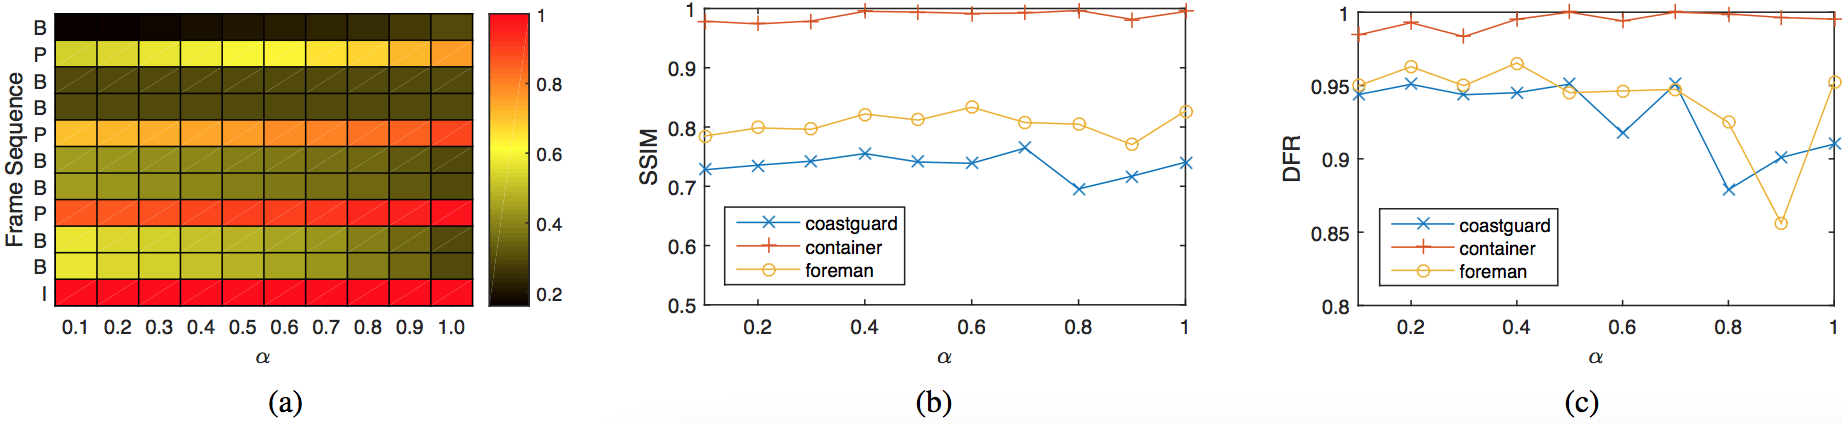
\includegraphics[width=1.0\textwidth]{Parameter_alpha}
  \caption{$\alpha$对权重影响,(a)PSNR,(b)SSIM,(c)DFR}
  \label{fig:parameter_alpha}
\end{figure}
\begin{figure}[H] % use float package if you want it here
  \centering
  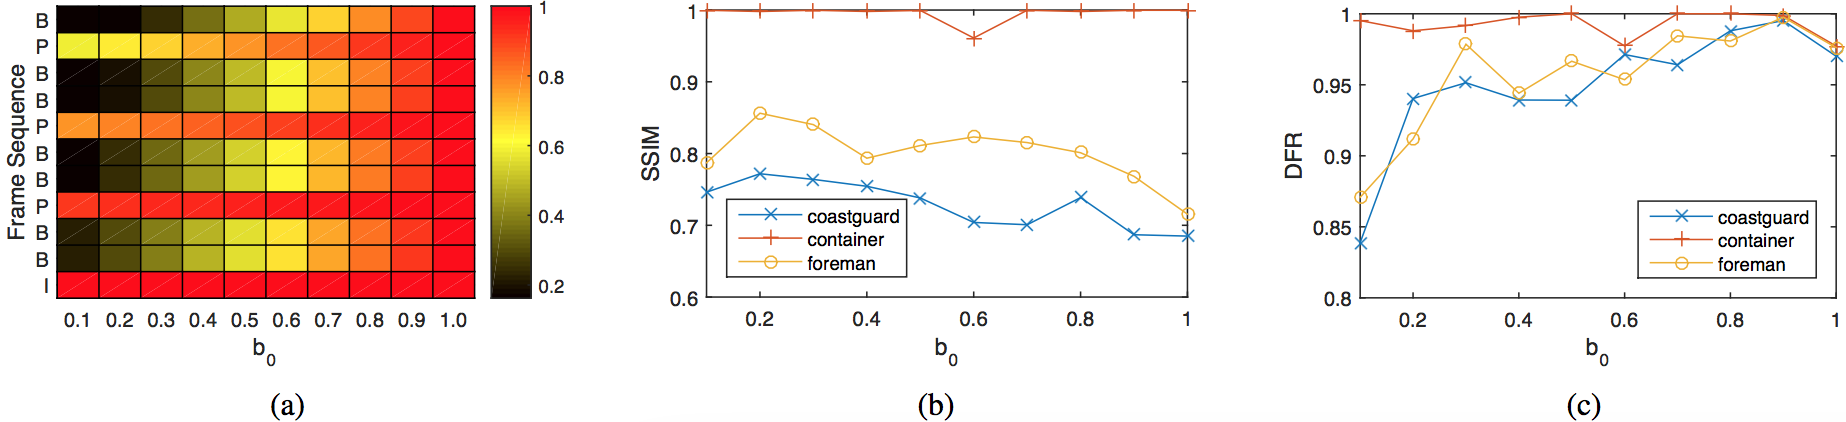
\includegraphics[width=1.0\textwidth]{Parameter_b0}
  \caption{$b_{0}$对权重影响,(a)PSNR,(b)SSIM,(c)DFR}
  \label{fig:parameter_b0}
\end{figure}
\begin{figure}[H] % use float package if you want it here
  \centering
  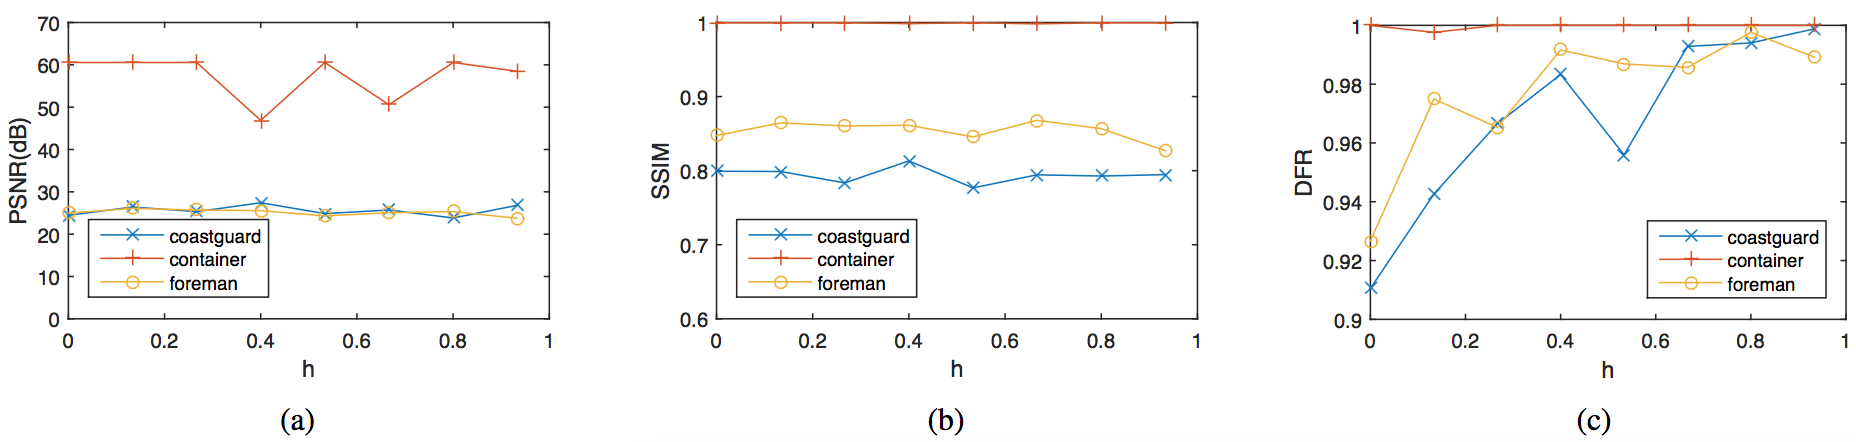
\includegraphics[width=1.0\textwidth]{Parameter_h}
  \caption{\emph{h}对权重影响,(a)PSNR,(b)SSIM,(c)DFR}
  \label{fig:parameter_h}
\end{figure}

\textbf{视频内容的影响}。实验结果在视频大小,时长,内容丰富性上有较大差异。比如,“container”
是一段监控视频,记录缓慢的桥梁的画面;相比之下,“coastguard”记录了一段摩托艇在海上冲浪
的视频,画面变化非常快,因此,在实时性上,“coastguard”的要求比“container”要高很多。从
图~\ref{fig:parameter_alpha},~\ref{fig:parameter_b0}和~\ref{fig:parameter_h}可见,
在任何情况下,无论上述的参数如何设定,“container”都可以以很高的质量呈现。所以,本文所
设计的映射算法在数据量大,延时要求高,丢包严重的场合更加能够体现其优势,也可以预期其在
复杂的工业监控场景下的良好的性能。


\section{路径质量敏感的动态切换阈值}
\label{sec:3}
无线Mesh网络目前还处在一个高速发展的阶段,不管是学术界还是工业界目前都还在尝试不同的技术。
物理层上,MIMO、多无线模块、软件无线电等技术都被尝试应用到Mesh网络中以获得更好的网络性能。
链路层上,QoS技术、时分复用技术等也被广泛应用。网络层上更是围绕组网协议这一核心功能集中
了大量的研究工作,在~\ref{sec:2.2}节中已经列举了诸多目前正在使用的Mesh组网协议,它们在链路选择、组网方式
上或多或少都存在差异,而这些协议目前共同面对的一项挑战就是移动场景下漫游的
切换时延问题。本节的工作集中在移动场景下如何保证客户端接入在不同的Mesh主干网络节点之间切
换时做到低时延。

在~\ref{sec:3.2}节中详细介绍了BATMAN-adv协议的数据包类型、节点发现过程、链路质量估算和路由
选择过程。其中链路质量的估算直接影响到链路的选择,决定了能否及时的感知链路状况变化,
客户端发生漫游,并且是切换链路的直接决定条件。但另一方面,如果对链路状态过于敏感,
则可能导致路由震荡,甚至路由失效。这些问题在后面的实验验证部分会通过实际场景论述。因此我们
需要在路由对链路变化感知敏感度和路由切换频率之间进行权衡。

如~\ref{sec:3.2.3}节所介绍,在BATMAN-adv协议中,TQ值作为链路估算的标准值,描述在链路上传输成功的
概率。TQ值记录在OGM包中,随着OGM传播至网络中其他节点,在传播过程中逐跳累乘当前链路TQ值,并
在每多一跳时减少一个惩罚值,该惩罚值默认为30,作为对多跳路径的惩罚,这意味着在网络构建
中偏向于选择尽量短的路径。TQ值存储为一个8位的数值,大小为0-255,数值越大表示链路的质量
越好,255即表示该路径上的数据可以保证百分之百的传输成功率。另外,TQ值在最终被使用时还会
经过一个滑动窗口做滑动平均,窗口默认大小为5,即对最近的5次计算得到的TQ值做滑动平均,
以此防止网络的抖动对路由选择造成影响,而链路的抖动在无线网路中十分常见。

因为节点无法直接计算发送的成功概率,所以在实现中通过接收质量RQ(从该邻居点成功接收的概率)
和回程质量EQ(成功发送至该邻居节点并成功收到应答的概率)得到。
计算过程在~\ref{sec:3.2.3}章节中详细介绍。
最终的单跳链路的TQ计算公式为$TQ=\frac{EQ}{RQ}$。整条多跳路径的TQ值为该多跳路径上每一条
单跳链路TQ值的乘积。

当链路质量能够支持所有的发送数据包都能够被接收方成功接收,则TQ值为最大的255。
相反,当网络中的链路质量出现波动,比如一条链路上出现遮挡或者节点移动,则此时链路的TQ值
下降,下降后的TQ值随着OGM广播至全网其他节点,接收到的节点做相应的路由表更新。
而如果在OGM广播到相应节点更新的这段时间内,节点正在进行通信就会出现通信中断,中断时长
视OGM的传播速度和相应节点路由表更新速度而定。
这就会引入一个
时间差。如图~\ref{fig:roming_1},一个客户端从之前接入的节点移动至另一位置,通过另一个Mesh
节点接入Mesh网络,客户端仍然能够和网络中的节点正常通信,因为网络中的每一个节点都会通过
接入点的OGM知道客户端的存在。然而,OGM的产生和传输需要一段时间,这段时差内,
网络中的其他节点仍然将传送至客户端的数据包交给之前的接入点,
而之前的接入点在这段时间差内也
同样不知道客户端的状态,所以实际上客户端是无法和网络中其他节点交互的。这段时差随
网络规模而变,在实验网络中可长达数秒,如图~\ref{fig:roming_2}这样的多跳场景,1号节点需要
6个OGM的转发周期才能获知客户端当前的接入状态,我们称之为\emph{多跳灾难},如果
在传输过程中任意一跳丢失会导致传输时间间隔成倍增长。这对于对时延敏感
的数据,尤其是VoIP或者视频监控数据是无法忍受的。

\begin{figure}[H] % use float package if you want it here
  \centering
  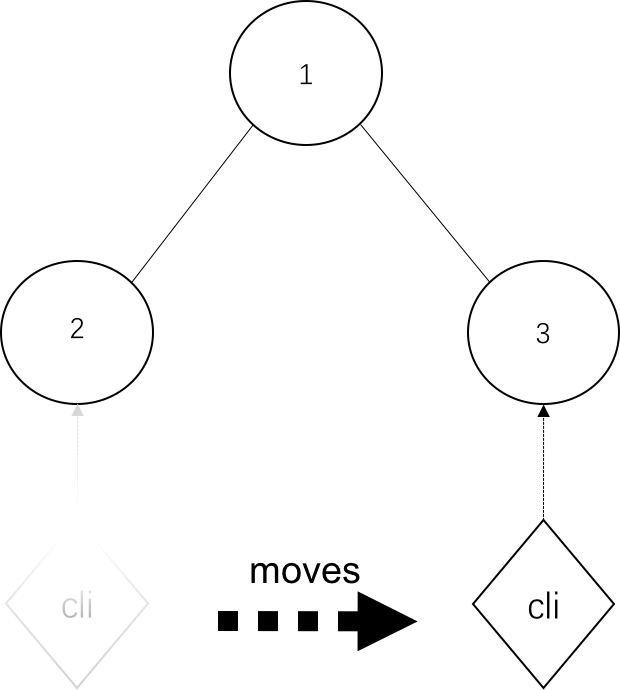
\includegraphics[width=0.3\textwidth]{Roming_1}
  \caption{无漫游机制下的节点接入点切换}
  \label{fig:roming_1}
\end{figure}
\begin{figure}[H] % use float package if you want it here
  \centering
  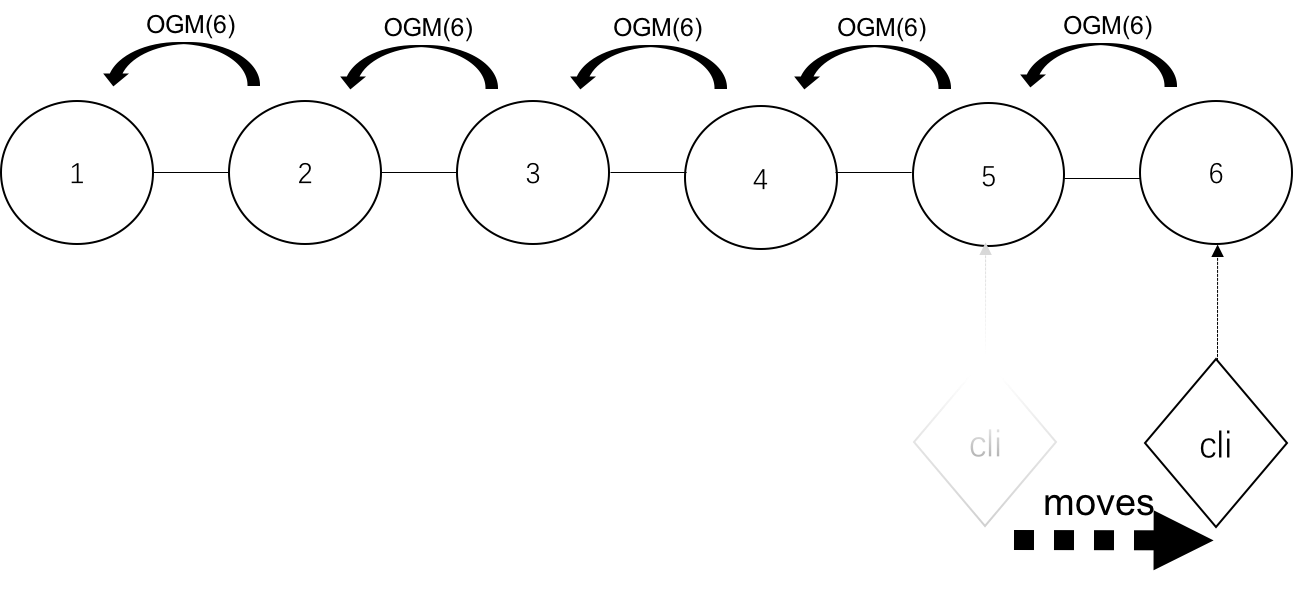
\includegraphics[width=0.6\textwidth]{Roming_2}
  \caption{多跳灾难}
  \label{fig:roming_2}
\end{figure}

\subsection{BATMAN-adv的漫游支持}
所谓\emph{漫游},指当客户端
在网络中移动,从一个接入点移动到另一个接入点的过程中不会失去连通性。传统的没有漫游技术
支持的网络,如上节所述,当客户端从一个接入点移动到另一个接入点,需要新的接入点通过OGM以广播的形式
通知全网中的其他节点客户端的接入状态,直到所有节点都获知客户端的接入状态变化才能够
确保客户端能够与网络中其他节点通信。而这个过程随网络规模的扩大而扩大,对于时延敏感
的应用场景无法忍受。

因此,BATMAN-adv在2011年引入了对漫游的支持。该机制的核心在于添加一种称为\emph{漫游
数据包}的包类型,当客户端移动到新的接入点,仍然能够充分利用原先已经建立的连接,即使此时原先
的连接已经不是最优的方案。

当一个节点检测到漫游事件时,就会发送一个\emph{漫游数据包},以快速恢复原先的连接。
那么如何检测到漫游事件呢?当节点检测到客户端接入时会首先检查当前路由表中是否有到达该客户端
的路由,如果有,则说明该客户端是从之前的接入点漫游过来的。如果要通过OGM包告知网络
中之前正在与该客户端通信的节点显然很困难,因为新的接入节点并不知道客户端之前的通信节点
有哪些。同时也无法保证有没有新的节点在寻求与客户端通信的有效路由。此时,比较有效的方法是
利用客户端之间的接入点已建立的有效连接。于是,新的接入点通过单播包的形式通知旧的接入点,
“客户端已经通过我接入网络”,该数据包即\emph{漫游数据包}。旧的接入节点就可以快速的建立
到达客户端的临时路由,网络中其他节点则可以暂时通过旧接入点和临时路由完成与客户端的通信。
这个阶段网络中的其他节点是不知道客户端发生了漫游的,但也不应该一直使用这条临时路由通信,
因为这条路由并不是协议选择的最佳路由。
所以,与此同时,新接入点的OGM包会广播通知全网节点客户端新的接入状态,在OGM广播全网完成
后,所有节点通过信的接入点重新建立起到达客户端的有效路由。

\begin{figure}[H] % use float package if you want it here
  \centering
  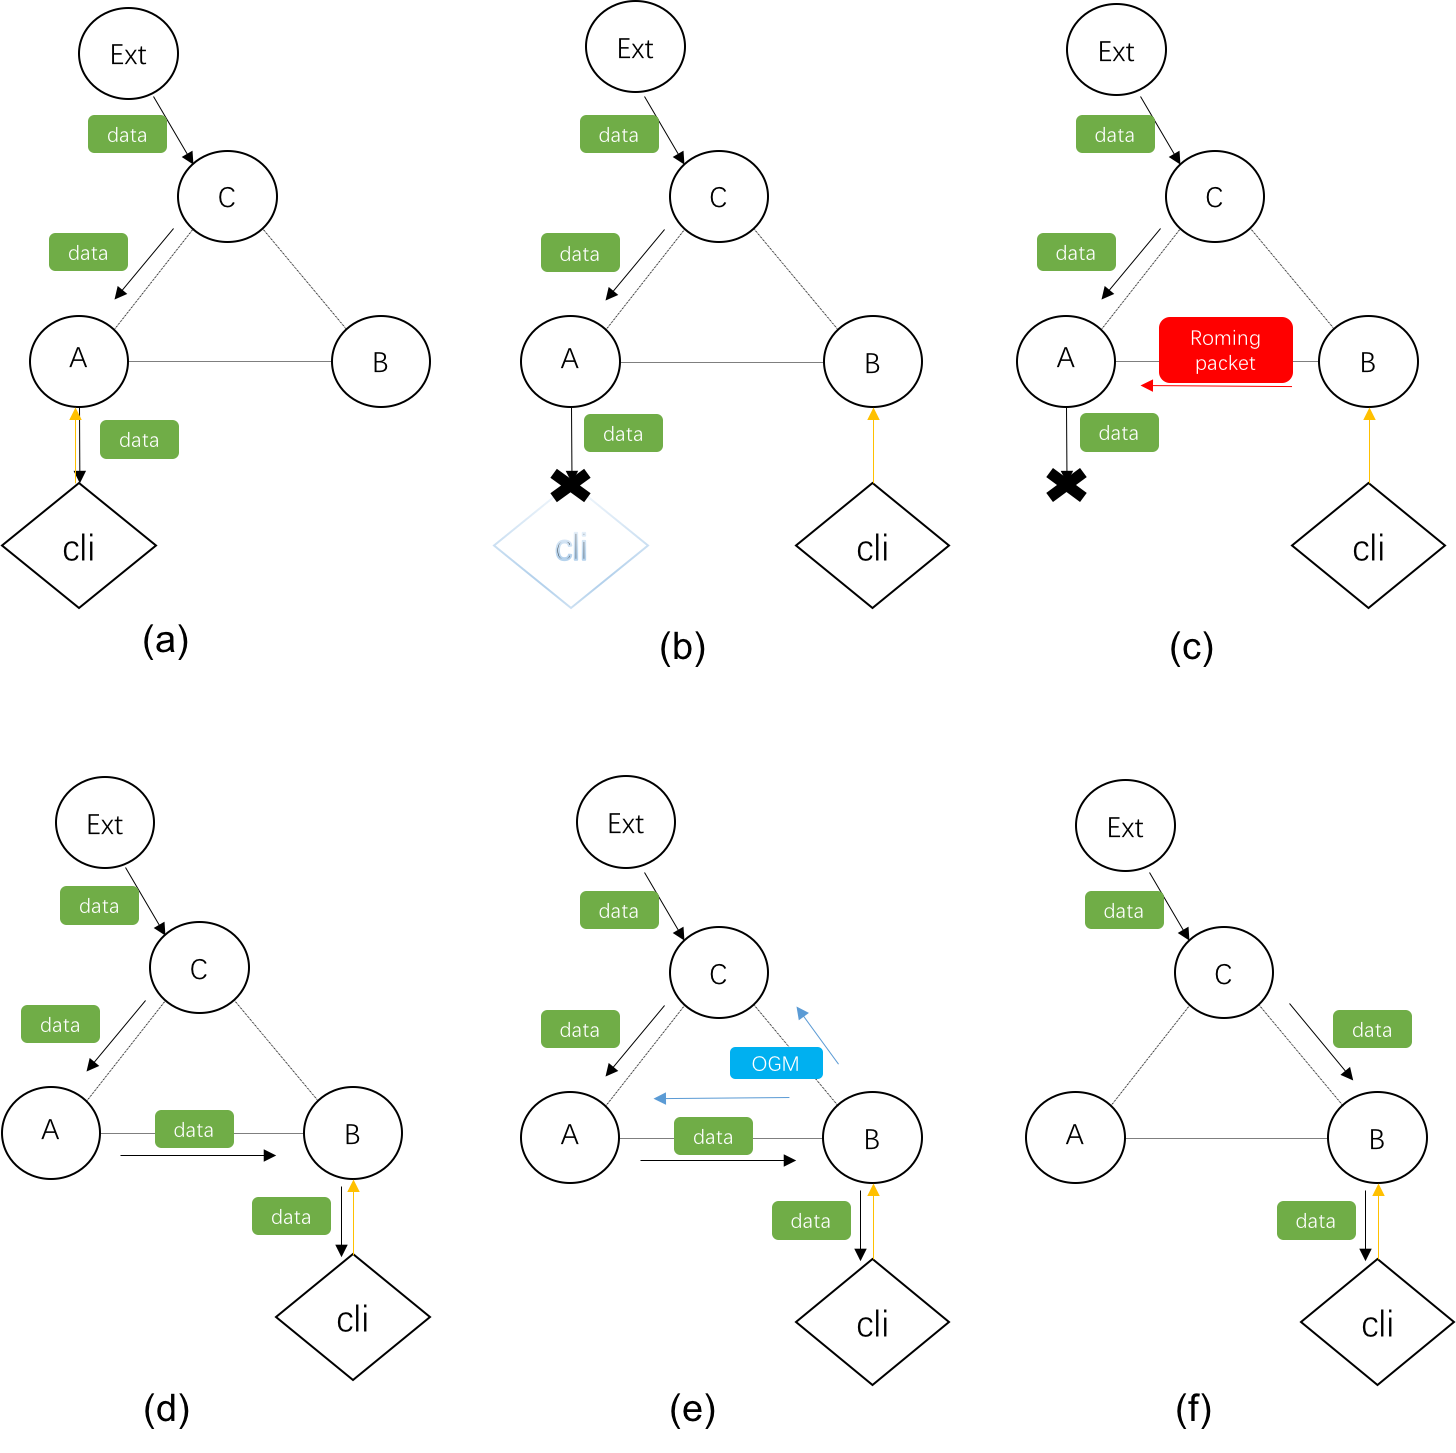
\includegraphics[width=0.8\textwidth]{Roming_3}
  \caption{客户端漫游,连接切换过程}
  \label{fig:roming_3}
\end{figure}

图~\ref{fig:roming_3}详细解析了客户端的漫游过程。
\begin{itemize}
\item[(a)] 客户端cli和ext之间建立有效路由,cli通过C节点和A节点接收来自ext的数据。
\item[(b)] 客户端cli从接如点B移动到接如点A,这个时间段内ext发送给cli的数据在A点丢失。
\item[(c)] 一旦cli与B点连接成功,B点就会发送一个\emph{漫游数据包},以单播包的形式发送
给A点。
\item[(d)] A点就开始将发送给cli的数据转发给B点。
\item[(e)] B点继续广播OGM至网络中的其他节点,其他节点更新cli的新的接入状态。
\item[(f)] 所有节点收到B点的OGM后就会构建新的有效路由,直接将发送给cli的数据交给B点而非
之前的A点。
\end{itemize}

\subsection{TQ值差异导致的切换延时}
BATMAN-adv引入的漫游机制很好的优化了客户端漫游的切换时延问题。但是,在实验中
我们发现,客户端在漫游的过程中并不是突然从一个接入点移动到另一个接入点,很多情况下
是在两个接入点之间逐渐过度,移动的过程中同时与A点和B点建立有效连接,
在选择路由时根据两条路径的
TQ值大小决定。在这样的场景下,如果两条路径的TQ值差异较大
,客户端从TQ值较大的接入点向TQ值较小的接入点移动就会出现长时间的连接中断或者
通信质量差。
下面的实验将进一步说明这一现象。

\renewcommand{\thesubsubsection}{\Alph{subsubsection}.}
\subsubsection{实验方法}
在固定位置放置三套Mesh节点,位置成一条直线,相邻节点相距100米。通过加装衰减器,调整功率
使得仅相邻节点可互相感知,1号节点和3号节点不能够直接通信,每个节点的有效信号覆盖范围
如图所示。此时在一辆车上放置一个节点,
节点同样控制在和固定节点相同的功率。3号节点连接一个摄像头,小车节点连接笔记本电脑实时
现实摄像头图像。实验过程如下:
\begin{itemize}
\item[1.] 车辆按图示方向从1号点出发到达3号点,再返回1号点。在这个过程中记录TQ值的变化,
当前路径条数以及视频质量变化情况。
\item[2.] 将TQ值计算的滑动窗口长度从5缩减到1,重复1的过程。
\item[3.] 将包OGM包发包频率从默认的1000ms调整为200ms,重复上述实验。
\end{itemize}

\begin{figure}[H] % use float package if you want it here
  \centering
  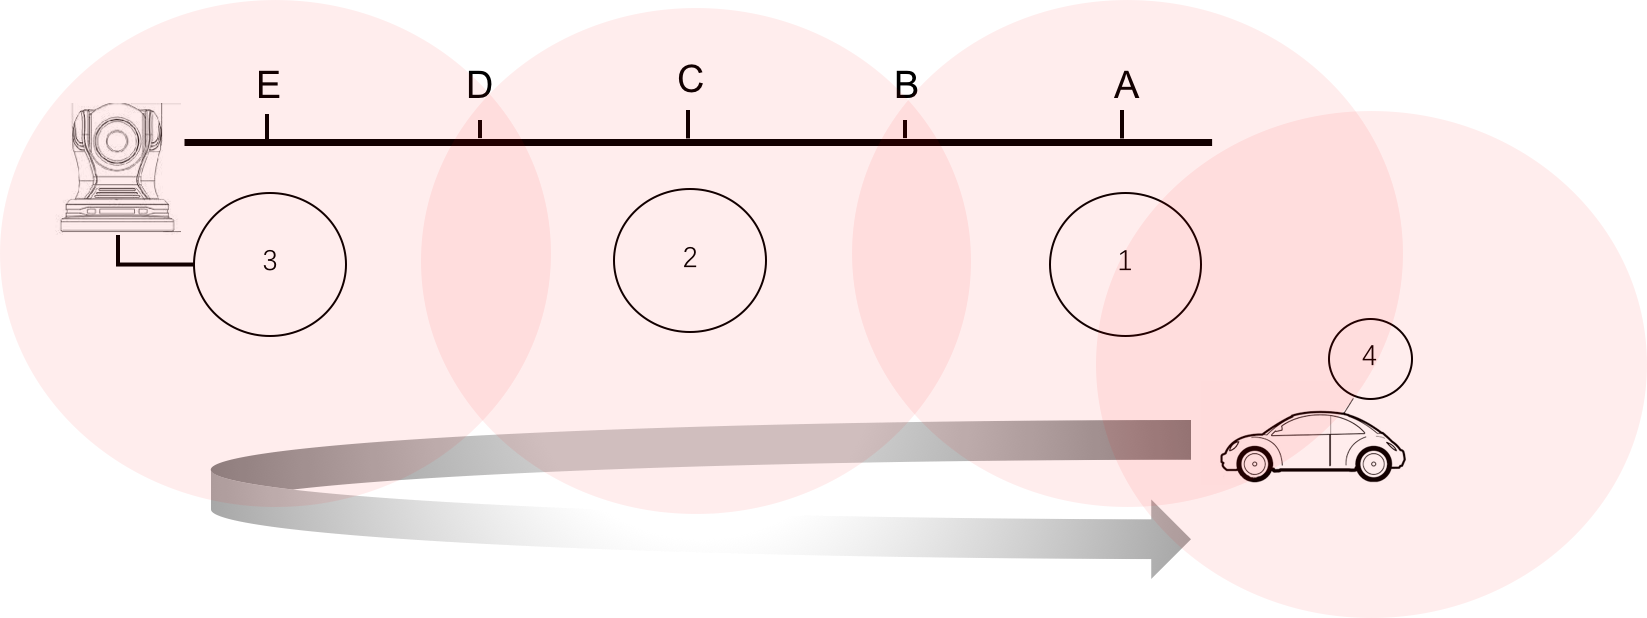
\includegraphics[width=0.8\textwidth]{Roming_4}
  \caption{链路切换实验图示}
  \label{fig:roming_4}
\end{figure}

\subsubsection{实现过程及现象}
\begin{itemize}
\item[(1)] 试验车从A点开始行驶,此时4号节点和3号节点之间通过3跳路径连接,4->1->2->3。
整条路径的TQ值为190,视频传输正常;小车前进至B处的过程中,3跳路径的TQ值逐渐减小。而此时
另一条可用的2跳路径,4->2->3的TQ值逐渐增大,当两跳路径的TQ值增大到超过3跳路径一定值时,
实际传输路径理解切换为2跳路径。
\item[(2)] 试验车继续驶离B点,驶向D点,2跳路径的TQ值继续增大,当试验车驶过2号节点后,
2跳路径的TQ值开始减小,与此同时建立其另一条有效单跳路径,4->3,且单跳路径的TQ值开始逐渐
增大,最终实际路由路径平滑切换到单跳路径。
\item[(3)] 之后试验车开始向反方向行驶,单跳TQ值逐渐减小,两跳路径(4->2->3)TQ值逐渐增大,
当试验车靠近2号节点时,\emph{视频断开连接}。经过30秒左右视频连接恢复。
\item[(4)] 试验车继续向A点行驶,2跳路径TQ值逐渐减小,3跳路径(4->1->2->3)TQ值逐渐增大,
当试验车靠近A点时,\emph{视频断开连接}。经过30秒左右视频连接恢复。
\item[(5)] 改变TQ值计算的滑动窗口大小会对实验效果产生影响,会显著加快TQ值的更新,
但窗口过小,比如设为1的情况下会造成负面影响,在网络不稳定的情况下导致TQ值变化剧烈。
\item[(6)] 改变OGM发包频率效果显著,TQ切换速度显著加快,实验中将OGM发包频率从1000ms
改为200ms,相应的试验车反向行驶到2号节点时,视频断开的时间间隔由30秒缩短为5秒。同样
的,当试验车反向行驶,靠近A点时,视频断开的时间间隔也缩短为4秒左右。
\end{itemize}
由以上实验我们发现当路径的切换是从长路径(跳数更多的路径)向短路径(跳数更少的路径)切换时,
可以达到完全的无缝切换;但是,当切换是从短路径向长路径切换时,\emph{通信会有一段时间的
断开}。另外,缩小TQ值计算的滑动平均窗口或增加OGM发包的频率均可以增强链路对TQ值变化的
敏感性,很大程度上增加切换的速度。

\subsubsection{实验结果及分析}
实验暴露的问题是,为什么从短路径切换到长路径会出现一段时间的通信中断。这个问题可以从
BATMAN-adv的路由选择算法得到答案。参考实验示意图~\ref{fig:roming_4},试验车回程过程中,
初始时,试验车与3号节点之间显然通过单跳路径(4->3)通信;当试验车行驶到D点时,两跳路径
(4->2->3)就成为一条备选路径,此时4号节点有两种路径选择,但此时会继续选择单跳路径
(因为两跳路径的TQ惩罚,此时单跳路径的TQ值会明显大于两跳)。此时单跳路径的TQ值显示为230,
然而由于TQ值更新的滞后性(为了减小网络抖动带来的影响),实际TQ值是小于230的;而两跳
路径的TQ值显示为225。

当试验车继续行驶,会出现这样一段时间:单跳路径的TQ值显示为225左右,然而因为TQ值更新
滞后,实际要远小于225(差值与试验车行驶速度有关),导致单跳路径无法正常通信。而两跳
路径TQ值也为225(因为需要减去30的多跳惩罚值,两跳路径的TQ值最大为225)。于是,即使两跳
路径的通信质量明显好于单跳路径,但由于TQ值无法及时真实地反应这个差异,也就存在这样一个
时间窗口无法正常通信。相反的,如果从长路径切换到短路径,就不存在这样一个时间窗口。
因为如果短路径能够支持正常通信,那么它的TQ值不会明显小于长路径,当长路径的TQ值衰退
到达一定程度就会触发路径切换。

至于缩短TQ值滑动平均窗口和增加OGM发包频率,虽然增加了链路切换的敏感性,但可能造成路径
切换频繁,在一些场景下可能链路质量波动频繁,导致链路切换频繁,进而导致网络无法提供
正常的数据传输功能。这也会成为网络遭受DOS攻击的一个隐患。

\subsection{路由切换优化}
在实验阶段已经尝试了两种解决方案,并做了分析,一种是缩减TQ值计算的滑动窗口,
另一种是增大OGM的发包频率,两者同样都会造成链路的抖动,导致无法提供正常的数据传输服务。
但是两种方法确实可以很好的提升路由切换的速率。
于是问题转化为如何在较小的滑动窗口和较高的OGM发包频率下减少路由抖动的产生?

BATMAN-adv在路由选择算法上考虑了路由抖动的问题。它的实现思路很简单,只有在发现一条路径
的整体QT值\emph{显著}优于当前使用的链路时才会切换到新的路径上。所谓\emph{显著}即存在
一个固定的\emph{切换阈值},只有当存在一条链路的TQ值高出当前链路TQ值至少\emph{切换阈值}
时才会进行链路切换。固定阈值的方法在一些场景下适用,但是也存在显著的缺陷,
如果阈值设得过低,则不能防止路由抖动;如果
阈值设得过高,那么当当前路径TQ值较低,以致不能提供良好的传输带宽时,
不能够及时切换到TQ值较大的链路上。那么能否找到
一个合理的阈值,在两者之间取得平衡呢?很遗憾,不存在这样的万能阈值,因为无线链路本身
受环境影响非常大,在不同的环境中,这个阈值的取值会千差万别。那么,如何设定一个
合理的路径切换机制呢?

面对上述问题,我们引入了新的动态路由切换指标。新的指标可以直接和TQ值衔接,
不需要改变现有TQ值的计算方法。目标是尽量选择质量较好的链路,同时尽量减少路由波动,维持
网络拓扑的稳定。
设新的动态路由切换指标为\emph{h}。\emph{h}和BATMAN-adv
中原先的切换阈值功能类似,但会随着TQ值和切换频度的变化而变化。

BATMAN-adv在进行路由决策时,如果是第一次建立此条路由,
则在路由表中选择TQ值最大的路径;如果已经存在一条正在使用的路径,则在路由表中查看,是否
存在TQ值\emph{显著}大于当前路径TQ值的路径,如果存在则替换当前路径,否则仍然使用当前路径。
引入\emph{h}后,路由决策算法为:如果第一次建立某条路由时,在路由表中选择TQ最大的路径;
如果已经存在一条正在使用的路径,
则在路由表中查看,是否存在TQ值超出当前路径TQ值至少\emph{h}的路径,若存在则以之替换当前
路径,否则仍使用当前路径。

具体的,\emph{h}定义如下:
\begin{equation}
\label{equ:h_threshold}
h = max\{a*\lfloor\log TQ\rfloor + b*\lfloor \log c\rfloor + h_{0}, h_{0}\}
\end{equation}
其中,\emph{c}为选择当前路径的频次,利用路由表项的留用字段存储,每次选择该条路径时加1。
$h_{0}$表示路径切换的最低阈值,可以理解为BATMAN-adv原来的切换阈值,但取值较低,作用仅在于
过滤因链路轻微的暂态波动干扰。在该式中,$\log TQ$
的取值范围为$-\infty < a*\lfloor\log TQ\rfloor \leq 8*a$,
$0 \leq b*\lfloor \log c\rfloor < \infty$。
而实际上,同一条路径切换频次在我们的统计数据中,均在10次以内,
$b*\lfloor \log c\rfloor$的取值范围在$0 \leq b*\lfloor \log c\rfloor \leq 3*b$的范围内。实验中,我们
取$h_{0}$为5,这样得到\emph{h}的取值范围为$[5, 8*a+3*b+5]$。公式中,两个取整项是为了和
BATMAN-adv的TQ值数据类型保持一致。

上述公式的实践解释如下:当当前路径TQ值较低时,意味着路径质量差,此时
会更加偏向于能够尽快的切换到通信质量较好的链路,
所以当TQ值低的时候,切换阈值\emph{h}较低,当TQ增大时,切换阈值逐渐增大,显然当TQ值较大时,也就是
说链路质量足够好,此时即使另一条链路质量有一个明显的优势,当前链路也足够承载数据量,
出于维持网络拓扑稳定的目的,尽量少的切换,此时切换阈值\emph{h}相应的较大。另一方面,
从切换频次的角度考虑,如果很少切换到当前链路,也就是当前链路的\emph{c}较低,有理由
相信可能是链路质量波动导致暂时的链路质量优势,倾向于选择其他更稳定的链路,于是切换
阈值\emph{h}自适应的调整为较低值;如果当前链路切换频次较高,也就有理由相信当前链路相对
较稳定的维持在高质量水平,倾向于不进行链路切换,于是切换阈值\emph{h}自适应的调整为较大。

\subsection{动态阈值实现}
\renewcommand{\thesubsubsection}{\Alph{subsubsection}.}
\subsubsection{BATMAN-adv结构}
BATMAN-adv是二层协议,作为一个Linux内核模块加在到系统内核。它作为网络栈中单独一层向
上层的网络层提供虚拟的Mesh接口,并向下层提供网络层接口。如图~\ref{fig:batman-structure}
所示。上层网络层只需要使用BATMAN-adv提供的接口,Mesh网络本身对网络层透明。同时下层使用
虚拟的网路层接口,同样不需要知道Mesh网络本身的存在。这就使得Mesh网络如同一个虚拟的
交换机,原来网络栈中的一切角色都只需要向其提供的接口发送数据,而不需要任何改变。
\begin{figure}[H] % use float package if you want it here
  \centering
  
\includegraphics[width=0.3\textwidth]{Batman-structure}
  \caption{BATMAN-adv结构示意}
  \label{fig:batman-structure}
\end{figure}

\subsubsection{BATMAN-adv主要功能模块及模块间交互}
BATMAN-adv模块载入系统内核并通过配置添加一个系统网络接口后,模块即完成注册,并开始接收
BATMAN-adv类型的数据包。相应的以太网类型和虚拟接口都完成创建。BATMAN-adv可以拆解为
很多个相互协作的功能模块,在图~\ref{fig:functions}中描述了它们之间的相互关系和数据
流向。
\begin{figure}[H] % use float package if you want it here
  \centering
  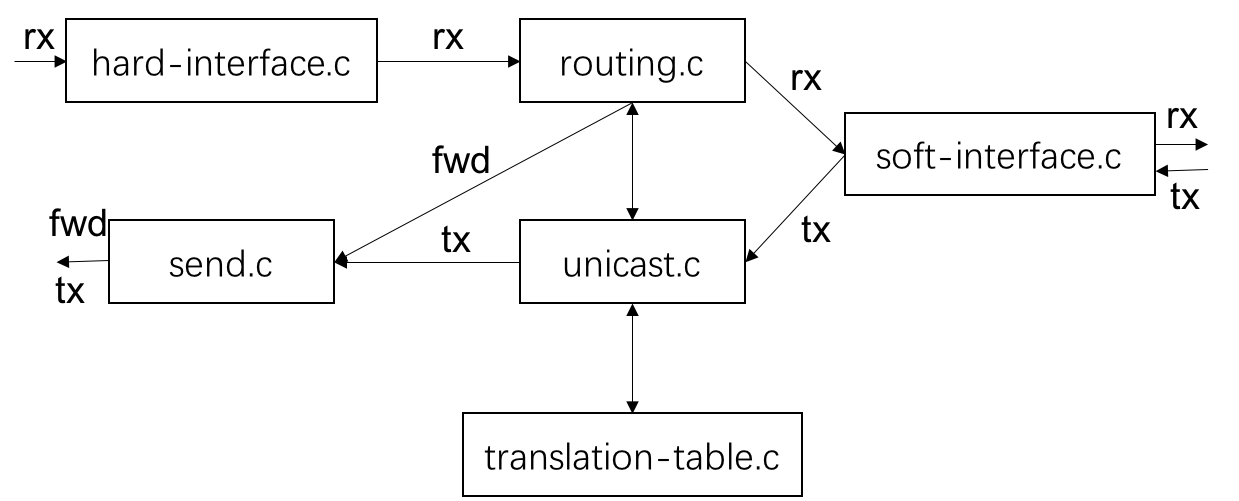
\includegraphics[width=0.7\textwidth]{Functions}
  \caption{BATMAN-adv功能模块}
  \label{fig:functions}
\end{figure}

\emph{soft-interface.c}模块中的函数使用虚拟网络接口。发送数据包时,数据包由
\emph{soft-interface.c}模块进入\emph{unicast.c}模块,\emph{unicast.c}模块将数据包进行
batman包头封装,从\emph{routing.c}模块获取路由信息,然后调用\emph{send.c}模块发送。

在\emph{hard-interface.c}模块中设置网络设备的回调函数。当网络设备的接收缓存中有batman类型数据时就
会触发\emph{hard-intervace.c}中的函数进行处理。模块接收到数据包后,转交给\emph{routing.c}
模块做进一步处理。如果这个数据包是需要转发的,就会进一步转交给\emph{send.c}模块。如果
是目的地址是自己,就会转交给\emph{soft-interface.c}模块。

\subsubsection{BATMAN-adv数据发送与转发}
每个BATMAN-adv节点需要维护
\textbf{Originators表}用以记录网络中所有BATMAN-adv节点。Originators表存储节点的信息,并
在转发和发送本地数据包时用来做辅助决策。同时每个节点还维护\textbf{邻居表}用以
记录所有的邻居信息,并在进行路由选择时选择最佳的邻居节点作为下一跳。另外,还需要维护
一个\textbf{转换表},用来记录非BATMAN-adv网络节点的设备的接入情况。

当节点需要发送数据时,首先查看目的地址是BATMA-adv设备,如果不是就查找转换表,找到该目的
设备连接在哪个Mesh节点下。然后以该Mesh节点作为目的节点进行路由。路由过程如下:
根据发送的目的节点地址搜寻Originator表,找到之后在确定到达目的
节点的最佳下一跳节点,然后在Neighbors表中找到该邻居节点,并将数据包发送给该邻居节点。
图~\ref{fig:function-send}给出了发送过程细致的函数处理过程。
\begin{figure}[H] % use float package if you want it here
  \centering
  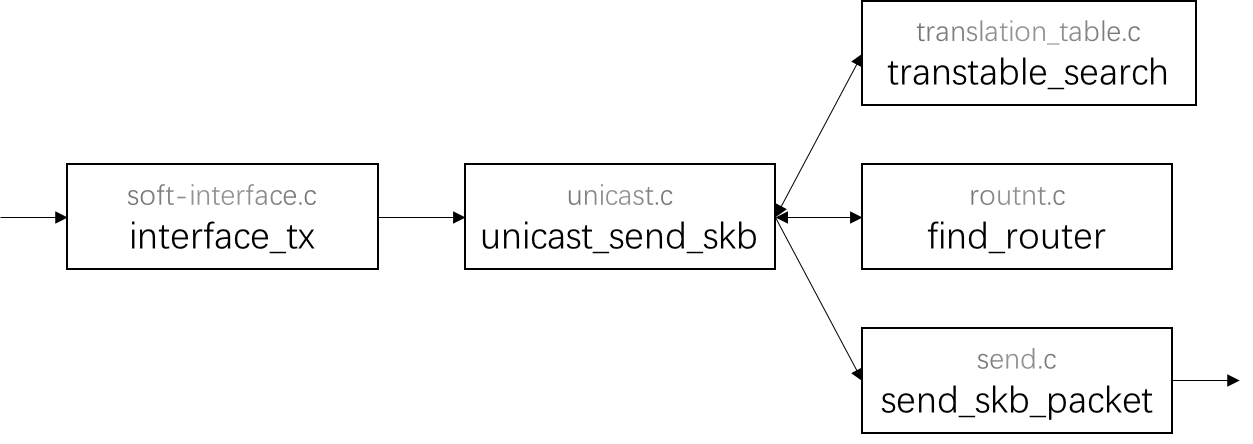
\includegraphics[width=0.7\textwidth]{Function-send}
  \caption{BATMAN-adv数据发送}
  \label{fig:function-send}
\end{figure}

协议栈中上层通过注册的回调函数$interface\_tx()$将数据交给BATMAN-adv。该函数会检查
源地址,如果该数据包来自一个新连接到节点的设备就需要在转换表中注册该设备的地址。
目的地址需要检查是否为单播包或者广播包,如果是单播报就交给
$unicast\_send\_skb()$,在该函数中搜索转换表查找目的节点。
然后,在\emph{routing.c}中查找到达目的节点的最佳下一跳邻居,并完成batman包头的封装。
之后交由$send\_skb\_packet()$进行发送。

\textbf{转发}和\textbf{发送本地}数据包,其流程十分相似,唯一的区别在于来源不同,
导致在预处理上有些许差异:转发
的数据包需要先判断数据包的类型,以及做一些路由环路侦测等处理;而本地数据包则直接从上层
虚拟Mesh接口获得,完成BATMAN-adv的封装。之后两种来源的数据包的路由和发送机制完全相同。

转发数据包从\emph{hard\_interface.c}模块进入,首先由$recv\_unicast\_packet()$函数
处理,检查源地址,如果本节点不是目的节点就将数据包交给\emph{routing.c}模块
由$route\_unicast\_packet()$函数完成路由和
包头数据的更替,之后交给$send\_skb\_packet()$完成发送。如果本节点是目的节点,数据包
就直接交给\emph{soft-interface.c}模块的$interface\_rx()$函数,进行batman包头剥离,并
传递给上层。

\subsubsection{BATMAN-adv中实现动态阈值切换}
考虑如何在BATMAN-adv中实现动态阈值切换,我们发现动态阈值切换主要的作用范围在于
单播包做路由决策时。当节点发送本地数据包或者转发数据包时,都会在发送之前选择最佳的
下一跳节点,也就是进行路由决策。如果之前没有在该路径上传输过数据,则需要从路由表中选择
最佳下一条,即TQ值最大的路径中的下一跳节点;如果之前传输过,此时针对该路径已经
存储了一个默认路由节点,这时进行路由决策就需要查看路由表项,是否存在某条路径的TQ值
显著优于默认路径,所谓显著就是说高出当前路径TQ值一定的阈值。

基于前面对BATMAN-adv功能模块的介绍,进行路由决策的模块为\emph{routing.c}。于是我们
深入\emph{routing.c}找到$bat\_iv\_find\_router()$函数,该函数中进行阈值比对。此处,
我们将原先的静态阈值替换为动态阈值,动态阈值通过独立模块计算返回。

综上,动态阈值切换的实现基于原BATMAN-adv的功能模块交互方式及数据流,增加了动态阈值计算
模块\emph{dynamic\_threshold.c},该模块和\emph{routing.c}模块交互,当\emph{routing.c}进行路由决策时,就会向动态
阈值计算时就会调用\emph{dynamic\_threshold.c}相关函数进行计算。另外,需要在路由表项的
数据结构中添加路径切换计数字段\emph{c},用以记录当前路径切换次数。添加动态阈值计算模块
后的功能模块结构如下图~\ref{fig:dynamic_threshold}
\begin{figure}[H] % use float package if you want it here
  \centering
  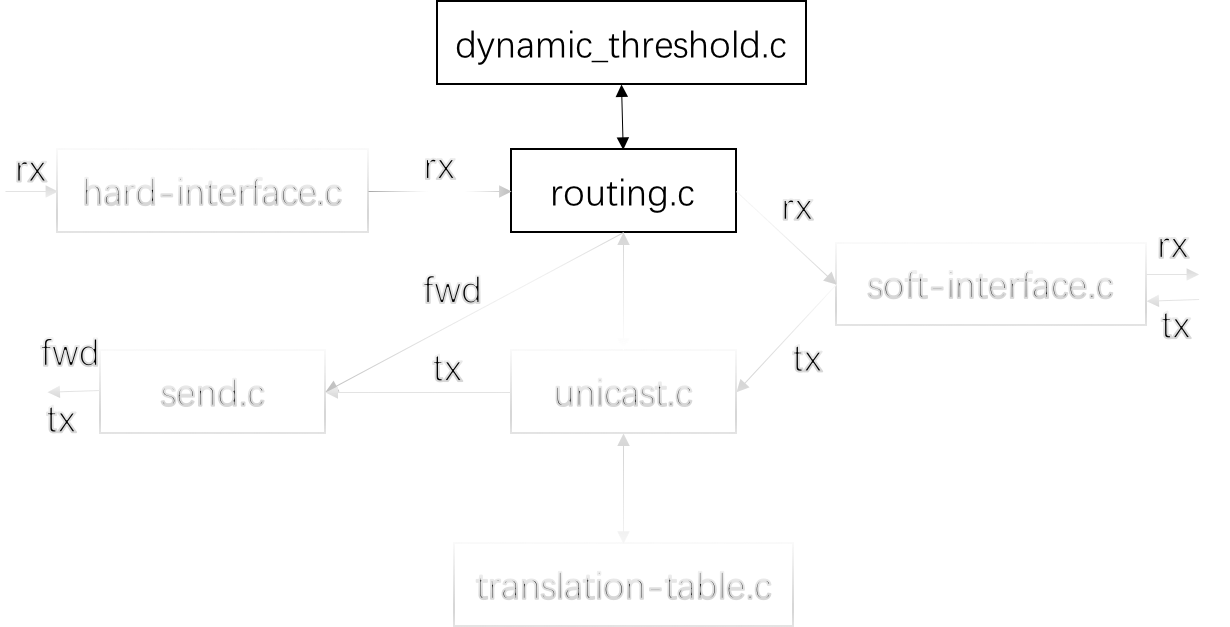
\includegraphics[width=0.7\textwidth]{Dynamic_threshold}
  \caption{动态阈值计算模块与BATMAN-adv交互图示}
  \label{fig:dynamic_threshold}
\end{figure}

至此就完成了动态阈值标量\emph{h}的设计与实现,那么它的实际效果如何我们通过如下实验加以
验证。

\subsection{实验验证}
\renewcommand{\thesubsubsection}{\Alph{subsubsection}.}
\subsubsection{整体性能}
实验的目的是验证该算法在路径TQ值相近
且频繁波动的情况下能否维持相对稳定有效的路由,以及公式~\ref{equ:h_threshold}中参
数的影响。该实验同样基于图~\ref{fig:realdeploy}示实际监控系统进行。

实验中将两个重要的影响参数进行设定,将TQ值的计算窗口长度从默认的5缩减到3,将OGM的
发包间隔从默认的1000ms缩减到200ms。
首先设定实验网络拓扑,如图~\ref{fig:roming_5}所示,1号点有两条有效路由可以和4号点通信,
通过2号点中继,或者通过3号点中继。在1号点上连接摄像头,那么4号点会通过1->2->4或者1->3->4
两跳路径收到摄像头的视频图像。此时如果在两条路径的第一跳上存在一个干扰物来回移动,
因为5GHz频段信号绕障碍的能力较差,当有障碍物移动到1号点和2号点之间时会影响1->2链路的通信
质量,降低1->2->4路径的TQ值,使得通过该条路径传输的视频图像卡顿;同样地,
当障碍物移动到1号点和3号点之间时会直接降低1->3->4路径的TQ值,使得通过该条路径传输
的视频图像卡顿。适当调节衰减器和发送功率,因为在实验设定中,TQ值的计算窗口和OGM的发包
间隔都缩短了,所以很容易达到如下状态:当障碍物移动到1->2链路上时,
BATMAN-adv会自动切换传输路径至1->3->4;反之,当障碍物移动到1->3链路上时,BATMAN-adv
会自动切换到路径1->2->4上。这样以一定的频率来回移动障碍物就会造成路由震荡,无法正常传输数据,视频
无法观看。而实际上,此时总是至少存在一条有效路径可以进行数据传递的。

分别对BATMAN-adv所使用的固定阈值和本章所提出的动态阈值算法做一组实验,每组实验以10秒
的周期来回移动障碍物,持续10分钟。实验中设定$h_{0}$为5。

\begin{figure}[H] % use float package if you want it here
  \centering
  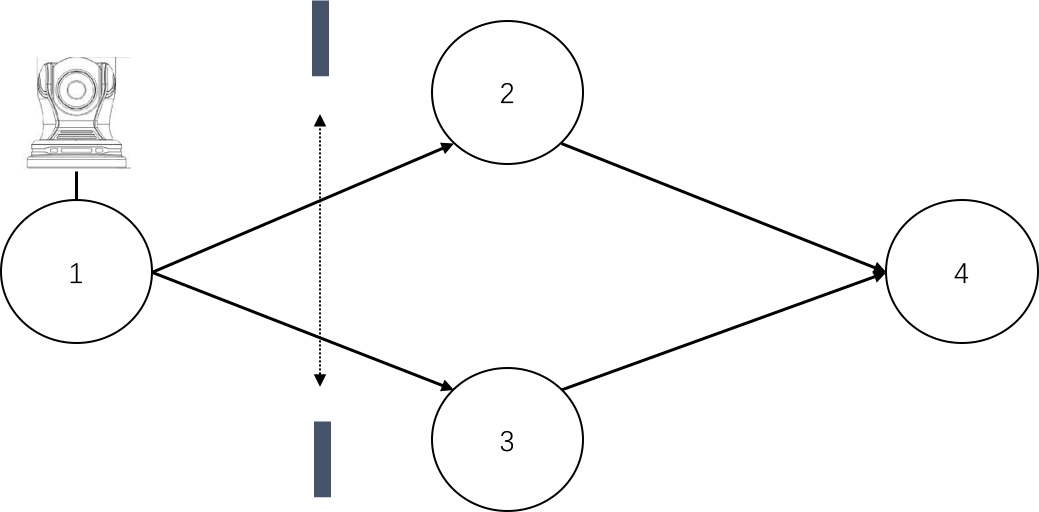
\includegraphics[width=0.6\textwidth]{Roming_5}
  \caption{路由震荡实验}
  \label{fig:roming_5}
\end{figure}

\begin{table}[htbp]
  \centering
  \caption{路由切换试验对比结果}
  \label{tab:roming_tab_1}
  \begin{tabular}{|p{3cm}|p{3cm}|p{3cm}|p{3cm}|}
  \hline
  路由切换算法 & 0-2分钟 & 2-5分钟 & 大于5分钟 \\
  \hline
  固定阈值切换算法 & 路由随着障碍物移动切换,成像不稳定 & 路由随着障碍物移动切换,成像不稳定& 路由随着障碍物移动切换,成像不稳定\\
  \hline
  动态阈值切换($a=2, b=3$) & 路由随着障碍物移动切换,成像不稳定 & 稳定成像 & 稳定成像\\
  \hline
  动态阈值切换($a=2, b=4$) & 短暂的震荡后稳定成像 & 稳定成像 & 稳定成像\\
  \hline
  \end{tabular}
\end{table}

\begin{figure}[h]
  \centering
  \subcaptionbox{}
      {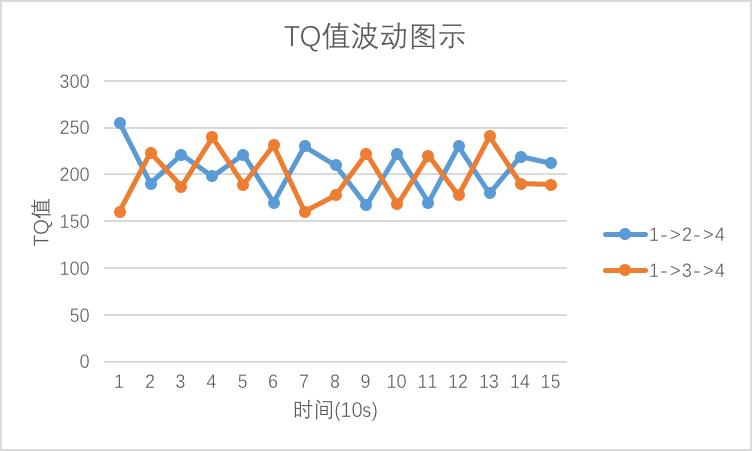
\includegraphics[height=4cm]{TQ_change}}
  \hspace{1em}
  \subcaptionbox{}
    {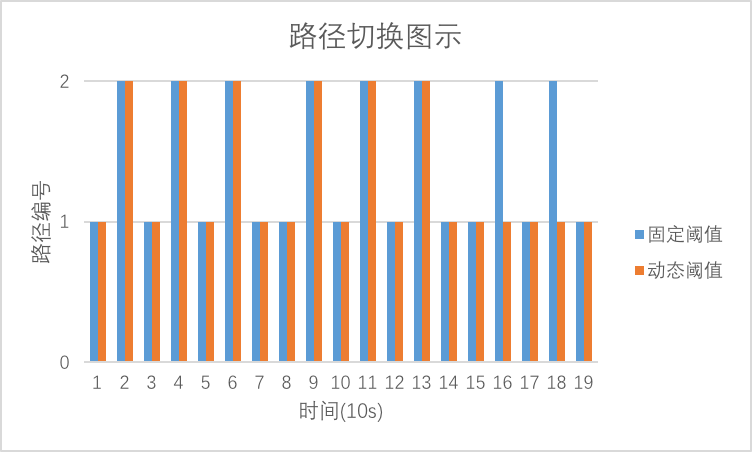
\includegraphics[height=4cm]{Route_change}}
  \caption{TQ值变化及路由切换对比}
  \label{fig:tq_route_change}
\end{figure}

实验结果如表~\ref{tab:roming_tab_1}所示。可以发现,引入动态阈值标量\emph{h}后,
前期(0~2分钟)路由抖动仍然存在,之后切换会越来越缓慢,且越来越少,最后一直维持在单一路由上。
结合公式~\ref{equ:h_threshold}分析如下:在整个实验过程中,两跳链路的TQ值都随着障碍
物的移动呈现周期性的波动状态,如图~\ref{fig:tq_route_change}(a)。
实验刚开始时,数据传输在1->2->4上进行,此时
链路1->2->4的\emph{c}值为1,链路1->3->4的\emph{c}值为0。当障碍物移动到1->2->4
路径上时,该路径的TQ值下降至低于路径1->3->4,于是传输路径切换至1->3->4。之后
当障碍物移动到另一条链路后,传输路径再次切换。值得注意的是,在整个实验过程中,
TQ值最差也不低于160,这个TQ值是可以保障我们实验中的视频稳定传输的,然而因为
路由频繁切换导致视频无法传输。在前两分钟内这个切换的过程对于
固定阈值和动态阈值的没有差异,都会导致路径近似于周期性的切换。但在这个过程中
动态阈值计算公式中的\emph{c}值在逐渐变大,当到达两分钟左右的时候,c值增大到
3,动态阈值此时的大小要比初始时高出$b*3$,这就保障了路径切换的标准增大,在
实验中表现为路径维持在路径1->3->4上。如图~\ref{fig:tq_route_change}(b)所示,
途中路径编号1为1->2->4,2为1->3->4。

另一个可能的疑虑是当TQ值不高,但因为频繁切换后\emph{c}值升高,导致动态阈值整体
较大,会不会导致此时即使出现一条TQ值很高的路径,仍然会受制于动态阈值而无法
切换呢?实际上,在实际实验中如果TQ值较,低那么\emph{c}值很难达到一个很大的值。假设
此时两跳路径TQ值较低,均在150以下,向同一条路径切换两次后该路径\emph{c}值为2。
此时动态阈值就会显著提高$b*2$,如果再次切换后TQ值必然已经达到一个较高的水平。

\subsubsection{各项参数对动态阈值的影响}
\textbf{参数影响之a}。\emph{a}的作用是根据TQ值的不同,调整动态阈值的大小。当
TQ值较小时,倾向于更快的切换到较好的链路上,因为此时链路无法很好的支持数据传
输。动态阈值变小会导致一定时间的路由波动的可能性,关于波动的抑制可以通过
\emph{c}值来调节。另一方面,当TQ值较大,此时显然链路足以支撑当前数据的
正常传输,因此倾向于保持在该条链路上,即使此时存在一个更好的链路也可以暂不考虑。
a取值偏小时会导致\emph{h}收敛速度慢,偏大则可能导致无法收敛到合理的值。
实践中一般建议取值范围为$\lbrack2,3\rbrack$。

\textbf{参数影响之b}。\emph{b}的作用是辅助\emph{c}值达到合理的收敛速度,
和\emph{a}类似,如果取值偏小会导致\emph{h}收敛速度慢,取值偏大则会导致\emph{h}
无法收敛到合理值。
实践中一般建议取值范围为$\lbrack4,6\rbrack$。


\textbf{参数影响之c}。\emph{c}的作用是当链路出现波动的时候起抑制作用,比如
当TQ值较小导致\emph{a}值较小进而导致链路波动时,在链路波动的过程中,每一次切换
相应链路上的\emph{c}值都会增加,而\emph{c}值的增加会带动动态阈值\emph{h}的
增加,从而抑制之后的链路切换。

值得注意的是,我们在公式中没有限定c值的范围,
在上一节也涉及过是否会出现c值较大导致链路停滞在较差水平而不进行切换。现做如下
讨论:因为TQ值最大为255,现假设TQ值从0开始向较高TQ值链路切换。初始阶段因为TQ值
和\emph{c}值均为0,所以只有$h_{0}$一项,假设$h_{0}$为5,也就是说此时的动态
阈值\emph{h}的值为5。那么当另一条链路TQ值大于5就会完成第一次切换,新的链路
动态阈值为大于等于$a*\lfloor \log 5 \rfloor$+5。
完成第二次切换后,新的链路动态阈值变为大于等于
$a*\lfloor \log(a*5+5) \rfloor$ +5。
当切换至之前的路径时,\emph{c}值大于等于2,$\log c$开始发挥作用。
新的链路动态阈值也就增加了$b*\lfloor \log c \rfloor$项。
假设\emph{a}取值为2,\emph{b}取值为3,那么在8次切换后,动态阈值\emph{h}的值
将达到25,而此时选择的链路质量也会显著好
于之前的链路。整个过程的各参数值变化参见表~\ref{tab:parameter_change},其中
最后一行的258加$*$号,为假设推导项。
因为TQ值最大为255,达到255后不再增加,所以也就不会再发生路径切换。从表中可以
看出动态阈值\emph{h}收敛于25,表中所推导的数据是再TQ值理想最低情况下,可以
判定动态阈值\emph{h}最高收敛值为25,收敛条件是TQ值接近255,亦可判定\emph{c}
值不会超过6。进一步地,当节点掉电或者其它原因导致某条链路从路由表中移除,重新
构建该链路后所有参数亦重新初始化。

\begin{table}[htbp]
  \centering
  \caption{参数变化表}
  \label{tab:parameter_change}
  \begin{minipage}[t]{0.4\textwidth}
  \begin{tabular}{p{2cm}p{2cm}p{0.5cm}}
  \hline
  TQ & c & h\\
  \hline
  0 & 0 & 5 \\
  5 & 1 & 9 \\
  14 & 1 & 11 \\
  25 & 2 & 17 \\
  42 & 2 & 18 \\
  70 & 3 & 20 \\
  90 & 3 & 20 \\
  110 & 4 & 23 \\
  133 & 4 & 25 \\
  158 & 5 & 25 \\
  183 & 5 & 25 \\
  208 & 6 & 25 \\
  233 & 6 & 25 \\
  258* & 7 & 28 \\
  \hline
  \end{tabular}\\
  \footnotesize *:假设推导项,实际$TQ \le 255$\\
  \end{minipage}
\end{table}

\textbf{参数影响之$h_{0}$}。$h_{0}$的作用和固定阈值相近,但它的主要目的是为了
在TQ值和\emph{c}都相对较小时,提供一个阈值的下限,加快收敛速度。所以它的取值
相对于固定阈值的设定也会相对较小。
实践中一般建议取值范围为$\lbrack5,10\rbrack$。

\section{本章小结}
本章详细介绍了系统的实际实现,尤其是本项目的三个核心创新点。

~\ref{sec:1}节针对无线信道干扰的问题设计了子网信道隔离的部署方案,将上百个节点组成
的全干扰网络划分为10个互相独立的子网,每个子网内自组织形成Mesh网络,上层通过
远距离无线传输设备将所有子网的数据通过簇首节点传输至汇聚节点。这样的网络规划可以
最大现大限度的发挥当前Mesh路由协议的承载能力,同时充分利用5GHz频段的频谱资源。
实现网络性能的巨大提升。实验显示,划分子网进行信道隔离后,原先近乎瘫痪的全干扰
网络可以流畅的传输所有30路高清视频数据。

~\ref{sec:2}节主要工作是设计了一种包级别的视频帧映射算法,用以提升在工业视频监控场景下的Mesh网络
视频传输性能。该映射算法综合考虑了多种对视频解码有影响的参数,如视频帧格式、视频帧
编码结构、帧序列以及头数据包的特殊性等,设计公式~\ref{equ:omega}综合以上参数,生成每个
数据包对应的权重。得到数据包权重后,结合队列的占用情况,将不同的数据包插入合适的发送
队列。最后,设计并实现了上述算法,在真实的系统中长期运行。相对于传统EDCA、静态映射算法
和动态映射算法,该映射算法在PSNR值上分别能够提升$>$50\%,16\%,5\%。

~\ref{sec:3}节首先从BATMAN-adv的路由算法及链路质量判定方法引出该路由机制在漫游场景
下对低延迟要求的服务无力支持的困境。随后介绍了一种优化方案,该方案中通过短暂的
复用之前建立的有效路由,完成路由重建的时间间隙中的通信需求,在这个时间间隔
中,所有到达漫游节点的数据由之前的接入点引导到当前接入点,从而完成通信。该方案
在瞬时漫游场景下表现良好,但是如果漫游节点在两跳链路之间缓慢移动,那么漫游
过程中的路径切换时延将无法避免。一个直观而有效的方法是缩减TQ值计算窗口,同时
减小OGM的发包频率。这两种方法都能够增加路由计算对链路质量变化的敏感度,从而
更快的在上述场景下完成路由切换。但是另一方面,增加链路敏感度可能导致路由震荡,
该现象往往出现在质量相近且波动频繁的链路之间。对于视频传输,路由震荡可能导致
视频卡断,甚至完全无法观看。同时存在遭受DOS攻击的风险。

针对这一问题,本章提出了一种新的动态阈值标量,定义为\emph{h},并在公式
~\ref{equ:h_threshold}中阐明其计算方法和意义。虽有通过实验对比动态阈值标量和
静态阈值之间的性能差异。实验显示,动态阈值的性能提升是巨大的。与缩短TQ值计算窗口和
提升OGM发包频率相结合,可以将实验场景下30秒的延时降低至4秒,同时有效抑制路由震荡,
最差情况下,路由震荡8次以内路径切换后进入稳态。

之后,讨论了公式~\ref{equ:h_threshold}中的参变量\emph{a}、\emph{b}、\emph{c}、
$h_{0}$取值不同对动态阈值\emph{h}的影响,影响主要是从收敛速度,确保收敛至合理
值等方面讨论,最后给出了不同参变量的合适的取值范围。


